%% How archival eclipse timing can produce period change
%% A&A regular article. Requires aa.cls (in this folder).
%% Figures expected in ./figures/ : fig1_barras.png fig4_dpdt.png fig2_v527_injecao.png fig3_cvdra.png fig5_completude.png
%% Generated from reports/dpdt_note.md by src/md_para_tex.py. Table bodies (Tables 3-5) come from the markdown
%% tables written by src/tabela_nota.py; preamble, captions, figure environments and bibliography are carried
%% verbatim from dpdt_note_v1.tex. Compile: pdflatex dpdt_note ; pdflatex dpdt_note
\documentclass{aa}

\usepackage[utf8]{inputenc}
\usepackage[T1]{fontenc}
\usepackage{graphicx}
\usepackage{txfonts}
\usepackage{rotating}
\usepackage[colorlinks,citecolor=blue,urlcolor=blue]{hyperref}
\usepackage{orcidlink}
\hypersetup{pdfauthor={R. Walitte}}

\renewcommand*\dblfloatpagefraction{0.85}
\renewcommand*\dbltopfraction{0.90}
\renewcommand*\topfraction{0.9}
\renewcommand*\bottomfraction{0.8}
\renewcommand*\textfraction{0.07}
\renewcommand*\floatpagefraction{0.75}
\setcounter{topnumber}{3}
\setcounter{bottomnumber}{2}
\setcounter{totalnumber}{5}
\setcounter{dbltopnumber}{3}
\hypersetup{pdftitle={How archival eclipse timing can produce apparent period change: Three mechanisms quantified on 26 short-period binaries}}
\begin{document}

\title{How archival eclipse timing can produce apparent period change}
\subtitle{Three mechanisms quantified on 26 short-period binaries}

\author{R.~Walitte\orcidlink{0009-0004-1776-2754}\inst{1}}
\authorrunning{Walitte}
\institute{Independent researcher, Rua 05, 76385-286 Goian\'esia, GO, Brazil\\ \email{rondinellewalitte@gmail.com}}

\date{Received ---; accepted ---}

\abstract{A quadratic ephemeris fitted to decades of eclipse timings returns a period-change coefficient whatever the data contain.}
{To quantify the three mechanisms on one sample, and to test the resulting coefficients against the complete TESS record of the same targets.}
{Timings of 26 binaries from TESS 2-min photometry and SuperWASP (2004--2008), with bars from the data, a null simulated as the pipeline operates, and 799 sectors of between-sector noise.}
{Formal photon-noise errors make 20 of these 26 targets significant, against 11 with data-derived bars; seven survive an admitted noise model, eight a 3-min archival offset, and all eleven a second timing template. Its residual test has a null of 0.77, and co-estimated bars overestimate $\sigma(\mathrm{d}P/\mathrm{d}t)$ by 2.9 at 0.2 s\,yr$^{-1}$. The complete TESS block \textbf{contradicts four of the seven coefficients it classifies} at more than 3$\sigma$ under every admitted model. Averaging primary and secondary minima bounds the anticorrelated component of spots, too loosely in six of eight; in the held-out V527 Dra, with a published orbit, the bound is 0.49 min peak-to-peak against a 7.3 min wander. Undersampled orbits account for N = 1.25 (95\% 0.80--2.46); the archival timing bias is $-$1.26 $\pm$ 0.75 min.}
{A quadratic coefficient fitted over 16--20 yr to a few epochs is a coefficient of its window: design and complete block are inconsistent in four of the seven the block classifies, which refutes a term common to both windows without electing a winner, and agree, with power, in one.}

\keywords{binaries: eclipsing -- stars: fundamental parameters -- methods: data analysis --
          methods: statistical -- techniques: photometric -- ephemerides}

\maketitle

\section{Introduction}\label{s:intro}
Secular period changes in close binaries encode mass transfer, angular-momentum loss and light-travel-time effects, but measuring them requires eclipse timings spanning decades, and the archival photometry that supplies the baseline comes with heterogeneous time systems, unquantified timing biases and no ground truth internal to the archive. A quadratic ephemeris fitted to a few epochs over such a baseline returns a coefficient whatever the data contain. That is the regime this paper is about: a handful of modern epochs, a couple of archival seasons sixteen to twenty years earlier, and a coefficient that the archival end carries almost by itself --- which is the regime most published period-change measurements are made in, and the reason the design here is held at four to seven epochs per target even where hundreds are available. This paper is about the ways that coefficient can be produced, and about how to tell.

Three mechanisms are quantified on one uniformly processed sample: timing errors that are formal rather than measured; timing bars that are estimated from too few samples and applied at another time-scale, where the question of \textit{whether} a bar is wrong is answered by a leverage-corrected decomposition of the residuals against the null of its own estimator; and third-body orbits sampled at a few phases, which a parabola absorbs into a coefficient that every internal test then certifies. The chain was developed on one system (TYC 7024-1046-1 = TIC 142874476), where a SuperWASP epoch from 2006--2008 propagated through a TESS-refined ephemeris sits 21.8 $\pm$ 2.2 min from the linear prediction, and is applied here to every catalogued binary for which the data allow the tests to run. The 26 binaries are the vehicle, not the object: they are the subset with data sufficient to demonstrate the mechanisms, drawn from a cache rather than from the sky (Sect.~\ref{s:sel}), and no population statement is made from them.

None of the three mechanisms is unknown. That formal photon-noise errors underestimate eclipse-timing uncertainties is why timing studies use the scatter of the data; that stellar activity puts structure into an O$-$C diagram is older still, whether as the quasi-cyclic period modulation of a magnetically active component (Applegate 1992) or as the timing noise that spots produce directly --- Tran et al. (2013) find O$-$C wander of 200--300 s in the close binaries of the Kepler field, anticorrelated between the primary and the secondary and attributed to migrating spots, in a sample an order of magnitude larger than this one, and Balaji et al. (2015) follow the spot longitudes that carry it; that a light-travel-time orbit sampled over a fraction of its period is degenerate with a quadratic ephemeris is a standing caveat of the eclipse-timing literature, stated wherever a cyclic and a secular term are fitted to the same O$-$C (e.g. Borkovits et al. 2016; Hajdu et al. 2019), and the timing of eclipsing binaries from TESS itself has been examined for exactly this degeneracy (Marcadon \& Prša 2024). What is new here is not the mechanisms but their measurement on one sample with one chain: a detection efficiency for undersampled orbits measured target by target at the real epochs with the real bars; one target with a published orbit and no secular term (V527 Dra) in which every internal test --- significance, adversarial, goodness of fit --- passes the confounder; a leverage-corrected decomposition of the residuals, with the null distribution of the estimator obtained by re-estimating the bars inside the simulation, which says whether either archive carries excess variance and --- in this sample --- traces an apparent archival excess to one estimation error measured against the wrong null and the remainder to three targets, rather than to the archive; and a test of the design inside the sample, in which the coefficient fitted to four epochs is confronted with the one the complete TESS block of the same target gives.


\section{The sample as a vehicle: 26 binaries with data sufficient for the tests}\label{s:sel}
Selection is deterministic and every cut is listed with its survivors (Table~\ref{t:funil}). The sample exists to run the tests of Sect.~\ref{s:val}, not to represent a population; the targets that were \textit{not} measured are nevertheless reported with the reason (Table~\ref{t:naomedidos}), because the guards that stopped them are part of the method.

\begin{table}
\caption{Selection funnel.}
\label{t:funil}
\centering
\begin{tabular}{c p{0.62\linewidth} r}
\hline\hline
Step & Criterion & N\\
\hline
1 & Union of the TESS eclipsing-binary catalogues of Prša et al. (2022; 4\,584) and Kostov et al. (2025; the 7\,936 systems new to that catalogue, its table 3; the 2\,065 previously known systems of its table 4 are not used), de-duplicated by position (5\arcsec) over the merged table & 12\,497\\
2 & Catalogue period P $<$ 5 d & 8\,759\\
3 & $\ge$ 2 TESS 2-min sectors separated by $\ge$ 1 yr among the 22 sector manifests held locally (s19--21, 27--28, 75, 90--105) & 288\\
4 & A SuperWASP source within 20\arcsec (public archive cone search --- the query that lists sources, not the light-curve download; 0 of 288 queries unresolved after retry) & 131\\
5 & $\ge$ 4 independent epoch clusters (TESS sectors + SuperWASP seasons), the minimum for a quadratic ephemeris with $\ge$ 1 degree of freedom & 88\\
6 & Passed all measurement guards (Sect.~\ref{s:met}) & \textbf{26}\\
\hline
\end{tabular}
\end{table}
Two remarks. The two catalogues are disjoint by construction (0 TICs in common; 23 positional pairs at 5\arcsec), so the union genuinely adds. And \textbf{the sector count of step 3 is a measure of our cache, not of the sky}: the 22 local manifests cover 21\% of TESS sectors, so 288 is a lower bound, and a biased one.

\textbf{The cache census.} The bias was measured rather than left as a caveat (\texttt{src/\allowbreak vies\_\allowbreak cache\_\allowbreak 288.py}; expectation written before running: a median ratio of 2--3 and 15--25\% of targets at a ratio $\ge$ 5). For each of the 288 targets that passed step 3, MAST was asked how many SPOC 2-min sectors exist (288 of 288 answered, 0 network failures). The cache holds a median of 4 sectors per target against an archive median of 32 (2--45), and 1\,224 sectors in all against 7\,857; the ratio has median 5.7, is $\ge$ 5 for 62\% of the 288, and rises with ecliptic latitude (Spearman +0.60, p = 5 $\times$ $10^{-30}$), from 2.3 at |$\beta$| < 40$^\circ$ to 10.0 at 78--90$^\circ$, where half of the 288 sit. The 26 measured targets are the extreme of this: ratio 10.5. The expectation was wrong by a factor of two in the median and three in the fraction above 5: the undercount is severe everywhere and worst exactly where the sample lives. Those 799 light curves are downloaded and used as the test of Sect.~\ref{ss:externo}.

What this implies is stated once and used throughout: this is not a sample of short-period binaries, it is a sample of binaries in the continuous-viewing zones with deep archival photometry --- which is what makes it adequate as a vehicle for the tests of Sect.~\ref{s:val} and inadequate as a population. The sky distribution of the result follows directly: 21 of the 26 measured targets are in Draco (the others: 2 in Microscopium, 2 in Grus, 1 in Indus), because the cached northern sectors overlap there and SuperWASP covered it in 2004--2008. The sample is a Draco sample with a southern tail, not an all-sky one --- which is why no population claim is made from it (Sect.~\ref{s:claim}).

\textbf{The design and the complete block.} The chain fits the design of four to seven epochs per target: the sectors already in the local cache --- a median of four per target --- plus the SuperWASP seasons. The 799 2-min light curves that MAST holds for the 26 are also used here, but in a different role: they are not folded into the design, they \textit{test} it. Four sectors per target is the regime in which the archival seasons carry the coefficient (Sect.~\ref{s:intro}), and keeping the design fixed is also what makes the tests of Sect.~\ref{s:val} comparable across versions of the chain; the complete block, 38 to 43 primary epochs per target over 2019.6--2024.9, gives an independent estimate of the same coefficient over the TESS window alone (Sects.~\ref{sss:teto} and \ref{ss:externo}). The epochs of the design are a subset of the complete block and are measured identically, so removing them from the block leaves a set that shares no epoch with the design: the test is repeated that way, and the classes it returns do not change (Sect.~\ref{ss:externo}).

\textbf{Where the block ends, and why.} The complete block stops at sector 86 (2024-12-18) for all eight targets that carry the test, and this is a pointing effect, not a cache effect: a MAST inventory of every time-series product of the eight (136--188 products each) returns nothing after s86, because the eight are in Draco (Dec +56$^\circ$ to +64$^\circ$) and TESS observed the south in 2025--2026 --- the control target at Dec $-$34$^\circ$ has sectors 97 and 105. An out-of-sample test with sectors later than the design is therefore not available today; its per-class prediction is registered in advance (Sect.~\ref{ss:externo}). For when those sectors arrive, the two full-frame-image reductions were compared with the 2-min epochs of the same sectors (s84--s86, 38 measurements, 200-s cadence): TESS-SPOC agrees with a median |t(FFI) $-$ t(2-min)| of 0.30 min and no systematic offset ($-$0.06 $\pm$ 0.16 min), while QLP does not (differences up to 7.2 min, and in s85 a shift of the same sign in all seven targets with a formal bar that does not cover it). TESS-SPOC 200-s photometry is usable for this timing; QLP needs a per-sector check against 2-min data.

\begin{table*}
\caption{\textbf{The 62 targets of the 88 that were not measured, by the first guard each one failed.} This table is a record of where each target stopped, not a map of what recovery would gain: every target fails at the first guard it meets, and behind the first there is usually another (see the recovery pass below). The ``Nature'' column describes the first reason only.}
\label{t:naomedidos}
\centering
\begin{tabular}{p{0.55\linewidth} c p{0.30\linewidth}}
\hline\hline
Reason & N & Nature\\
\hline
SuperWASP curve with $<$ 500 valid points after cleaning & 22 & archive depth; structural\\
Phase coverage of the eclipse not testable in $\ge$ 1 season block (Sect.~\ref{ss:barras}; a season whose fitted depth is $\le$ 0 counts as not testable, Sect.~\ref{ss:epocas}) & 22 & archive sampling; recoverable with a second archive\\
SuperWASP light-curve download returned an empty file in four attempts (a different operation from the cone search of Table~\ref{t:funil}, step 4) & 4 & archive-side failure; recoverable if the archive serves the file\\
Cycle count between TESS sectors ambiguous (period ladder did not close) & 8 & local sector coverage; intermediate sectors were added from MAST and none was recovered (per-target outcome in the deposit)\\
No applicable eclipse duration in the catalogue (4 NaN; 1 contact-binary width; 1 W UMa) & 6 & catalogue gap; $T_{14}$ was measured on the TESS curve for five and none was recovered (per-target outcome in the deposit)\\
\hline
\end{tabular}
\end{table*}
A recovery pass was run after the main batch on the two rows a local action could change (intermediate TESS sectors for the ladder row; eclipse durations measured on the TESS curves for the duration row) and recovered none of them: behind the first guard there was a second in every case, so recovery is not additive across the rows of Table~\ref{t:naomedidos} and the count of 26 stands (the per-target outcome of the recovery pass is deposited as \texttt{reports/apendice\_\allowbreak a\_\allowbreak recuperacao.md}). The 26 are therefore not a random sample of short-period binaries: they are the subset with deep SuperWASP coverage, eclipses sampled in every season, and unambiguous cycle counts across the sectors held locally.


\section{Method}\label{s:met}

\subsection{Eclipse epochs}\label{ss:epocas}
For each TESS sector we fit a periodic trapezoid of free depth to the PDCSAP light curve (QUALITY = 0, normalised to the 95th percentile) on a fine grid of trial epochs, with the eclipse duration $T_{14}$ from the catalogue and the period from the catalogue, seeded on the catalogue reference epoch so that the primary is fitted rather than the deepest minimum in the curve (in contact systems these differ). The epoch is the $\chi^2$ minimum; the formal error is the $\Delta\chi^2$ = 1 half-width. Sectors are anchored to the most recent one.

For SuperWASP we convert HJD\_UTC to BJD\_TDB (a +1.1 min shift at these dates --- larger than the TESS timing error), fit the same profile per observing season, and require phase coverage of the eclipse in every season ($\ge$ 50 points in eclipse, no empty phase bins in 12). A season whose fitted depth is $\le$ 0 is rejected: the grid has found a $\chi^2$ minimum for a \textit{brightening}, and its ``epoch'' is not that of an eclipse. Five of the first 31 targets had such a season; their between-season dispersion was 82 min against 1.8 min for the rest.

\textbf{Blending.} A constant neighbour in the aperture dilutes the depth of an eclipse and does not move its time of minimum; only a neighbour that is itself variable on the time-scale of the eclipse can shift a minimum or add timing structure. What can be measured cheaply is who has a neighbour capable of it (\texttt{src/\allowbreak blending\_\allowbreak 26.py}; expectation written and committed before running). The SPOC crowding metric CROWDSAP of the 84 sectors used has a median of 0.97 per target (median over its sectors), 14 of the 84 sectors are below 0.9 and none below 0.5; the lowest is TIC 377253090 (0.56 in all four sectors). Gaia DR3 sources within 48\arcsec (about two TESS pixels) and within 2 mag in G of the target exist for three of the 26: TIC 229476285 (18.8\arcsec, $\Delta G$ = 1.5), TIC 359552377 (10.1\arcsec, $\Delta G$ = 1.9), and TIC 377253090, a member of D9, which has a companion of nearly equal brightness at 1.7\arcsec ($\Delta G$ = 0.37) that neither TESS nor SuperWASP resolves: which of the two stars is the eclipsing binary, and whether the other is variable, is not decided by the data of this paper, and the detection is carried with that caveat. No blending correction is applied to any epoch, since none is needed for a constant neighbour; the variability of the neighbours was not tested.


\subsection{Period ladder and cycle count}\label{ss:escada}
Within the TESS sectors the period is refined by a ladder: starting from the two closest sectors, each further sector is added only if its linear residual stays below a tolerance equal to the larger of 3 min and three times the median epoch uncertainty of the target (3 min for 22 of the 26; 3.2--5.5 min for the other 4), and the result is discarded if shifting any epoch by $\pm$1 cycle does not worsen $\chi^2$. The ladder returns epochs and residuals in the caller's order (Sect.~\ref{s:val}).

The ladder is \textit{not} used across the 2008--2019 gap: it requires a linear ephemeris, and a real $\mathrm{d}P/\mathrm{d}t$ produces tens of minutes of O$-$C over 19 yr, which the ladder would reject as an unresolved alias. Across the gap the cycle number is the rounded propagation with the TESS-refined period, and the count is accepted only if $\sigma_P \times N$ < 0.25 cycle at the farthest epoch. Any target with $|\mathrm{d}P/\mathrm{d}t|$ > 10 s\,yr$^{-1}$ is flagged as a suspected cycle-count error rather than a measurement; none of the 26 is.


\subsection{Timing uncertainties from the data}\label{ss:barras}
The formal $\Delta\chi^2$ = 1 error is a photon-noise error. Cycle-to-cycle eclipse-timing scatter from spots and O'Connell-type asymmetries is not in it, and in the SuperWASP data the dispersion between observing seasons exceeds the formal error by a median factor of 4.3 (n = 25 targets of the 26; one record lacks the formal value; interquartile range of the factor 2.9--10.7). We therefore assign each epoch the \textit{larger} of its formal error and the dispersion between independent subsets: the two halves of the sector for TESS, the observing seasons for SuperWASP. Each SuperWASP season enters the fit as its own epoch with this error --- the dispersion of one season, ${\rm std}(d)$, not the standard error of the season mean, ${\rm std}(d)/\sqrt{n}$, which is the bar of the \textit{combined} epoch used on the control target; an earlier version assigned the latter to each season (Sect.~\ref{sss:decomp}, Appendix~\ref{a:C}) --- added in quadrature to the chain-bias uncertainty of Sect.~\ref{ss:vies}. A target with a single valid season has no red-noise estimate and is not measured. Where the archive holds one observing season only, the season is split at its midpoint into two blocks of 39--43 nights and the bar is the dispersion between the halves (as for TESS): this is the case for five of the 26 (TIC 229461186, 229476285, 229914020, 230386284 and 424461577, all with two 2008 blocks 0.11--0.12 yr apart), whose ``two seasons'' in Table~\ref{t:coef} are two halves of one, and whose archival lever is a single epoch at 2008.5 rather than two seasons years apart. Two properties of these bars are shown by the data: because each is estimated from two or three samples that also enter the residual, the residual test has a null below 1 that must be simulated rather than assumed (Sect.~\ref{sss:nulo}), and the TESS bar, being a within-sector quantity, cannot contain timing drift between sectors (Sect.~\ref{sss:teto}). For TESS the bar is max(formal, $|t_a - t_b|/2$), with t\_a and t\_b the epochs fitted to the two halves of the sector: each half has an error $\sqrt{2}$ larger than the whole sector, so the difference of the two, divided by 2, estimates the error of the whole-sector epoch (a simulation of two halves with known scatter recovers the whole-sector error with $|t_a - t_b|/2$ and overestimates it by $\sqrt{2}$ with $|t_a - t_b|/\sqrt{2}$). The halves term sets the bar in 22 of the 84 TESS epochs and the formal error in the other 62. The divisor was $\sqrt{2}$ in an earlier version --- the dispersion of \textit{one half} given to the whole sector; the correction and what it moved are in Appendix~\ref{a:C}. The control target does not use the halves rule (its bar is the spread between three reductions; Appendix~\ref{a:A}) and reproduced before and after.


\subsection{SuperWASP timing bias}\label{ss:vies}
There is no ground truth internal to the archive, so the timing bias of the SuperWASP chain is calibrated on transiting hot Jupiters --- objects whose clocks do not run. Eclipsing binaries cannot serve: a first attempt with three gave an astrophysical O$-$C scatter of 31.7 min against 1.73 min for the hot Jupiters. The candidates are the 35 transiting planets with a SuperWASP source in the archive; all 35 have a published ephemeris built with ground-based timings, 15 yield a usable SuperWASP-era epoch, and 6 pass the between-season dispersion guard. The run that fixed the bias used four of those six (WASP-18 b, WASP-4 b, WASP-19 b and WASP-6 b, in the order used below), because it had been given the twelve highest-signal candidates rather than all of them; the other two, WASP-17 b and WASP-98 b, are measured in this version and reported below. Six is where the archive ends.

The calibration used here compares those four seasons with \textbf{ephemerides that include ground-based timings} rather than with a TESS-only propagation (\texttt{src/\allowbreak vies\_\allowbreak hj\_\allowbreak indep.py}): the homogeneous transit-timing ephemerides of Ivshina \& Winn (2022) and the ExoClock III ephemerides of Kokori et al. (2023), and for WASP-4 b the quadratic ephemeris of Bouma et al. (2020), which rests on the TESS timing series of Bouma et al. (2019) and whose published period derivative is propagated with its own uncertainty (the covariance is not published, so the propagation is diagonal). The four O$-$C are $-$2.38 $\pm$ 1.08 (WASP-18 b), $-$0.81 $\pm$ 1.45 (WASP-4 b), +0.46 $\pm$ 2.59 (WASP-19 b) and +0.40 $\pm$ 1.85 min (WASP-6 b), with the ephemerides of Ivshina \& Winn (2022) and the Bouma et al. (2020) term on WASP-4 b, consistent with a constant offset ($\chi^2$ = 2.4 for 3 d.o.f.):

\begin{equation}
\text{chain bias} = -1.26 \pm 0.75\ \mathrm{min}.
\end{equation}
The two ephemeris sources agree to 0.03--0.40 min per season and give weighted means from $-$1.26 to $-$1.56 min; the propagated ephemeris uncertainties are 0.05--0.29 min, negligible against the 1.0--2.6 min of the archival seasons. The value is 1.7--2.1$\sigma$ from zero. A TESS-only propagation gives $-$2.14 $\pm$ 0.78 min, and the difference is almost entirely WASP-4 b, whose published orbital decay the TESS-only propagation folds into the bias ($-$2.55 min there, $-$0.81 min here).

Three candidate mechanisms for a bias of this size were tested and none reproduces it. (i) \textit{Shape.} A procedural bias arising in the fitting, the sampling or the profile is shape-dependent, and the four calibrators are shallow, long transits while the targets are deep, sharp eclipses. Transits of the published geometry were injected into the real SuperWASP curves of the four and measured by the same chain (\texttt{src/\allowbreak vies\_\allowbreak forma\_\allowbreak swasp.py}): the weighted O$-$C is $-$0.10 min (95\% interval $-$2.8 to +2.4), i.e. the offset of the earlier, TESS-only calibration is not reproduced by the estimator acting on the transit shape. The same injection on the eclipse shapes of the 26 gives per-target biases of up to $\pm$3 min, driven by template mismatch combined with asymmetric phase coverage --- so a \textit{common} bias is not what the estimator produces, while a \textit{per-target} one of a few minutes is. Since this version that correction is applied by the chain: each target's archival epochs are shifted by its own measured shape bias and the floor of the archival bar carries the uncertainty of that measurement (state (F) of Appendix~\ref{a:C}). The corrections are small where they matter --- at most 0.80 min in the eleven detections, 2.93 min in the sample (TIC 329248002) --- and the coefficients move by a median of 0.05$\sigma$ and at most 1.11$\sigma$ (TIC 126945917, which is not a detection before or after). No detection verdict and no flag changes; the class column of Table~\ref{t:coef} changes in two targets (TIC 126945917 and 329289186), in both because $p_{\rm curv}$ crosses 0.05, and in neither does the target become a detection --- the adversarial gate rejects both. The values before and after are in Appendix~\ref{a:C}. Three targets (TIC 139256217, 229476285 and 359552377) have a shape test that does not converge and are left uncorrected, with a 3 min floor instead. What the correction does not carry is the part of the shape bias that varies from season to season. Its direction is known even though its size is not: a per-season scatter enters the dispersion from which the archival bar is estimated, and by the coupling of Sect.~\ref{sss:secular} a larger bar \textit{suppresses} the significance of whatever term is there, so the omission works against detections and not in their favour. Its size is bounded from above by the sensitivity run of Sect.~\ref{sss:teto} and Appendix~\ref{a:D}, which imposes on every target's archival block a common offset of 3 min --- the largest per-target bias the shape test finds. (ii) \textit{Time system.} Twenty raw archival timestamps were converted independently with astropy and compared with what the chain produces (\texttt{src/\allowbreak checa\_\allowbreak tempo\_\allowbreak swasp.py}): the two agree to 0.002 s on average and 0.019 s at worst, so no sign error or missing term in the HJD\_UTC $\rightarrow$ BJD\_TDB conversion contributes. (iii) \textit{The calibration sample, and how far the archive takes it.} The four were not a chosen four, and the choice that produced them is worth stating plainly: the calibrator table is ordered by the signal-to-noise of the transit in the archival curve, and the run that fixed the bias took the twelve highest of the 35 --- a cut made for the cost of downloading light curves, not for any property of the objects, and made in a session rather than by a versioned script. Re-examining all of them (\texttt{src/\allowbreak calibradores\_\allowbreak expandido.py}) adds WASP-17 b and WASP-98 b and ends there: \textbf{the calibration now uses every object the archive allows}, which is a different statement from the one this paragraph carried before.

With six, the weighted mean is -1.66 $\pm$ 0.72 min against the Ivshina \& Winn ephemerides ($\chi^2$ = 5.8 for 5 d.o.f.) and -1.68 $\pm$ 0.71 against ExoClock III ($\chi^2$ = 2.6 for 5), against $-$1.39 $\pm$ 0.75 and $-$1.56 $\pm$ 0.74 with four. \textbf{The chain keeps the value of the four, $-$1.26 $\pm$ 0.75 min, in this version}: the six-calibrator mean sits inside its uncertainty, so the two are not in disagreement, and replacing it would move all 26 coefficients for a value that is not statistically distinct from the one they were computed with. What the larger sample does change is the limitation. With four, dropping WASP-18 b --- the most precise of them --- left $-$0.46 $\pm$ 1.04 min, compatible with zero: the bias rested on one calibrator. With six it leaves -1.08 $\pm$ 0.97 (-1.07 $\pm$ 0.96 with ExoClock). \textbf{That dependence does not survive the expanded sample}, and the declared limitation of earlier versions is withdrawn on this point.

\textbf{An empty join looks exactly like a complete one.} One methodological remark belongs with the calibration sample, because it is the sharpest instance of this paper's own subject. Matching the candidates to the two ephemeris catalogues keyed on the planet name; one of the two indexes by system instead, so that catalogue matched nothing, and the first pass computed the bias from the other alone --- returning a weighted mean, a $\chi^2$, a drop-one sensitivity and a count of eligible objects that were all correct for the set it had, and all silent about the set it had lost. An empty join looks exactly like a complete one unless the matches on each side are counted, which is now done and asserted (\texttt{src/\allowbreak calibradores\_\allowbreak expandido.py}; the entry is item 26 of the deposited record). The failure is not that a wrong number was published --- none was --- but that a right number for the wrong set is indistinguishable from the right answer at every point where a person would look.

The bias is subtracted from every SuperWASP epoch and its uncertainty added in quadrature. The calibrators the cap rejects --- between-season bars of 17 to 1\,682 min --- are not discarded silently: a calibrator whose seasons disagree by tens of minutes carries no information on a 2-min bias, and the guard was a cap of 5 min on the between-season bar. That cap is a calibrator rule and is \textit{not} applied to the targets --- a target keeps whatever between-season bar its seasons give it, and a large one simply removes it from the curvature test (the two targets with $\varepsilon$ = 0 in Sect.~\ref{ss:orb} have archival bars of 157 and 359 min).

\textbf{What the bias does to the results.} Its effect was measured rather than assumed, by refitting the 26 with the bias set to 0, $-$1.26, $-$1.56, $-$2.14 and $-$4.28 min and its uncertainty to 0.75 and 2.14 min (\texttt{src/\allowbreak sensib\_\allowbreak vies\_\allowbreak 26.py}). The verdicts are nearly insensitive: D11 keeps all eleven members at the adopted value and at zero, and loses two only at $-$4.28 min or with the bias bar inflated to 2.14 min; TIC 198408416, 232634196, 329246824 and 392536812 --- the four with the smallest relative uncertainty among the detections --- survive every diagonal combination; the goodness-of-fit flags never change. The \textit{values} are not insensitive: between a bias of 0 and $-$4.28 min the coefficient moves by more than its own $\sigma$ in 16 of the 26 (median 1.36$\sigma$, maximum 4.70$\sigma$), so the bias is a first-order term in the tabulated $\mathrm{d}P/\mathrm{d}t$ and a zeroth-order term in the verdicts. Choosing the ExoClock ephemerides instead ($-$1.56 min) changes no verdict at the adopted bias bar.

\textbf{A second template, with the width free.} The bias above is a property of one estimator: a trapezoid whose duration is taken from the catalogue and held fixed while the epoch is fitted. Everything this paper does about shape --- the per-target correction, the scan over a common archival offset, the conservative 3-min cut of Sect.~\ref{sss:teto} --- exists because that template can be wrong, so the first-order check is to fit another one and compare epochs. The same SuperWASP curves, the same season splitting and the same seed were refitted with the width free as a third parameter (\texttt{src/\allowbreak estimador\_\allowbreak alt\_\allowbreak d11.py}), on the 11 detections. The catalogue width is systematically too narrow: the free fit prefers 1.30 times it in the median and up to 2.2 times, and only one of the 11 prefers a narrower profile. The epochs, however, barely move. Season by season the difference has a median of 0.64 min and a 90th percentile of 4.91, with the largest (10.0 min) in the smallest season of the set; on the archival epoch that carries the lever --- all seasons together, which is what the chain fits --- the shift is 0.54 min in the median and at most 3.27 min. That is the behaviour a symmetric template has: its centre is insensitive to its width to first order, and what the width error buys is a wrong depth and a wrong bar, not a wrong time.

The comparison has to be made where the chain works. Each SuperWASP season enters the fit as its own epoch (Sect.~\ref{ss:barras}), so the quantity that propagates is not the shift of the combined archival epoch but the shift of each season, and those are larger: a 90th percentile of 4.91 min against three detections that a common archival offset of 2 to 2.5 min already removes (Table~\ref{t:coef}). An argument is available --- a \textit{common} offset is the form maximally degenerate with curvature, while season-to-season shifts of varying sign are much less so --- but the alternative epochs exist, so the argument is unnecessary. Each archival epoch was displaced by the shift measured for its own season and the eleven were refitted with the same machinery, the same bars and the same adversarial gate (\texttt{src/\allowbreak estimador\_\allowbreak alt\_\allowbreak refit.py}). \textbf{All 11 of the 11 detections survive}, with $p_{\rm curv}$ and $p_{\rm adv}$ below 0.05 as before; the coefficient moves by a median of 0.11$\sigma$ and at most 0.93$\sigma$ (TIC 329246824, whose worst season shifts by 10.0 min). The conclusion of the sample does not depend on which of the two profiles measures its archival epochs, and this is a refit rather than a bound on one.

Two of the 24 seasons have no measurable free width --- the fit runs to the edge of the width grid, in TIC 144194304 and TIC 198388252 --- and are reported as such rather than clipped to the edge. They enter the refit unshifted, so for those two targets the check is \textbf{partial}: what is verified is that the remaining seasons do not move them. Neither is among the three detections that a 2 to 2.5 min common offset removes --- both sit at 7 min --- so the fragile end of the sample is covered in full.

\textbf{Declared limitation.} The $\pm$0.75 min is a floor. The transfer of a bias measured on WASP planets --- the best-covered objects in the archive --- to eclipsing binaries is asserted, not demonstrated, and the shape test above shows the estimator can bias a \textit{given} target by a few minutes in either direction. The only eclipsing-binary check available is the data-level overlay of Sect.~\ref{ss:externo} (two SuperWASP-era epochs of CV Dra against independent CCD minima, differences $-$1.1 $\pm$ 2.7 and +2.8 $\pm$ 2.6 min): consistent with the transferred bias, and far from a measurement of it. One asymmetry of that check is worth stating, because it is the same term behaving in two ways: there the common-mode term does not cancel, since each epoch is compared with an external minimum rather than differenced against the target's other seasons, so a 3 min common offset widens those two comparisons to $\pm$3.9, 3.9 min, while in a fit the average over a target's seasons reduces it and $\sigma(\mathrm{d}P/\mathrm{d}t)$ of TIC 232634196 barely moves. One more thing the $\pm$0.75 min is not: independent from one season to the next. Added in quadrature to each epoch, as the tables do, it averages down by $\sqrt{n}$ over a target's seasons, whereas the uncertainty of a chain bias is a common offset of the whole archival block --- the shape most degenerate with curvature. The fits were therefore repeated by generalised least squares with that term moved from the diagonal into a common block over each target's SuperWASP epochs (\texttt{src/\allowbreak gls\_\allowbreak vies\_\allowbreak 26.py}): no verdict changes in any of the 26, no new detection appears, and $\sigma(\mathrm{d}P/\mathrm{d}t)$ grows by a median of 2\% and at most 16\%. The tables keep the diagonal treatment; the correlated one is the correct propagation and changes nothing that is claimed. The residual test of Sect.~\ref{sss:nulo} cannot bound any of this: a bias common to a target's seasons is a common offset of the archival block, which the quadratic absorbs, leaving no residual --- an earlier version of this paragraph claimed the opposite (Appendix~\ref{a:C}).


\subsection{Fit and tests}\label{ss:testes}
Linear and quadratic ephemerides are fitted by weighted least squares to all epochs (TESS sectors + SuperWASP seasons). $\mathrm{d}P/\mathrm{d}t$ = 2Q/P with Q the quadratic coefficient. Degrees of freedom are N $-$ 3; a target with N < 4 would be ``measured, not tested'' (none of the 26 is). Curvature significance is $\Delta\chi^2$ between the two fits with one degree of freedom.

Three tests accompany every number. The \textit{goodness of fit of the quadratic ephemeris} is the $\chi^2$ of the fit with its N $-$ 3 degrees of freedom, reported as $p_{\rm gof}$; a fit with $p_{\rm gof}$ < 0.05 is flagged ``parabola inadequate'' and its coefficient is not quoted as a rate. The level is the same as that of the curvature test, chosen for consistency and not for what it marks; an earlier draft used a fixed $\chi^2_{\rm red}$ $\ge$ 2, which corresponds to a false-flag probability that depends on the degrees of freedom (0.157 at 1 d.o.f., 0.135 at 2, 0.112 at 3, 0.092 at 4) --- the counts under both rules are reported in Sect.~\ref{s:res}. The \textit{curvature test} is the $\Delta\chi^2$ above. The \textit{adversarial test} shifts every epoch by one sigma in the direction that most weakens the curvature and reports the resulting p-value; curvature is called only if p < 0.05 both before and after. The shifted value is not a p-value --- a coherent one-sigma shift of every epoch has no null distribution --- and the test is a robustness heuristic, used here as a gate and not as a significance level. Its conservatism is not quantified analytically, but the rate that matters is measured by injection: over the 26 designs, with the bars re-estimated inside each realisation, the gate fires on noise alone in 0.0\% of realisations at the median target and the summed rate over the sample is 0.39 expected detections (Sect.~\ref{sss:secular}). Sect.~\ref{s:val} shows what it does and does not protect against.


\section{The chain applied to the 26}\label{s:res}
This section records what the chain returns with the data-derived bars of Sect.~\ref{ss:barras}, before any of the tests of Sect.~\ref{s:val}. Table~\ref{t:coef} is the per-target record on which Sect.~\ref{s:val} operates; Table~\ref{t:dist} summarises it in three partitions. Neither is a population result: the coefficients are quadratic coefficients over 16--20 yr, and Sect.~\ref{s:val} shows what they survive.

\begin{figure}
\centering
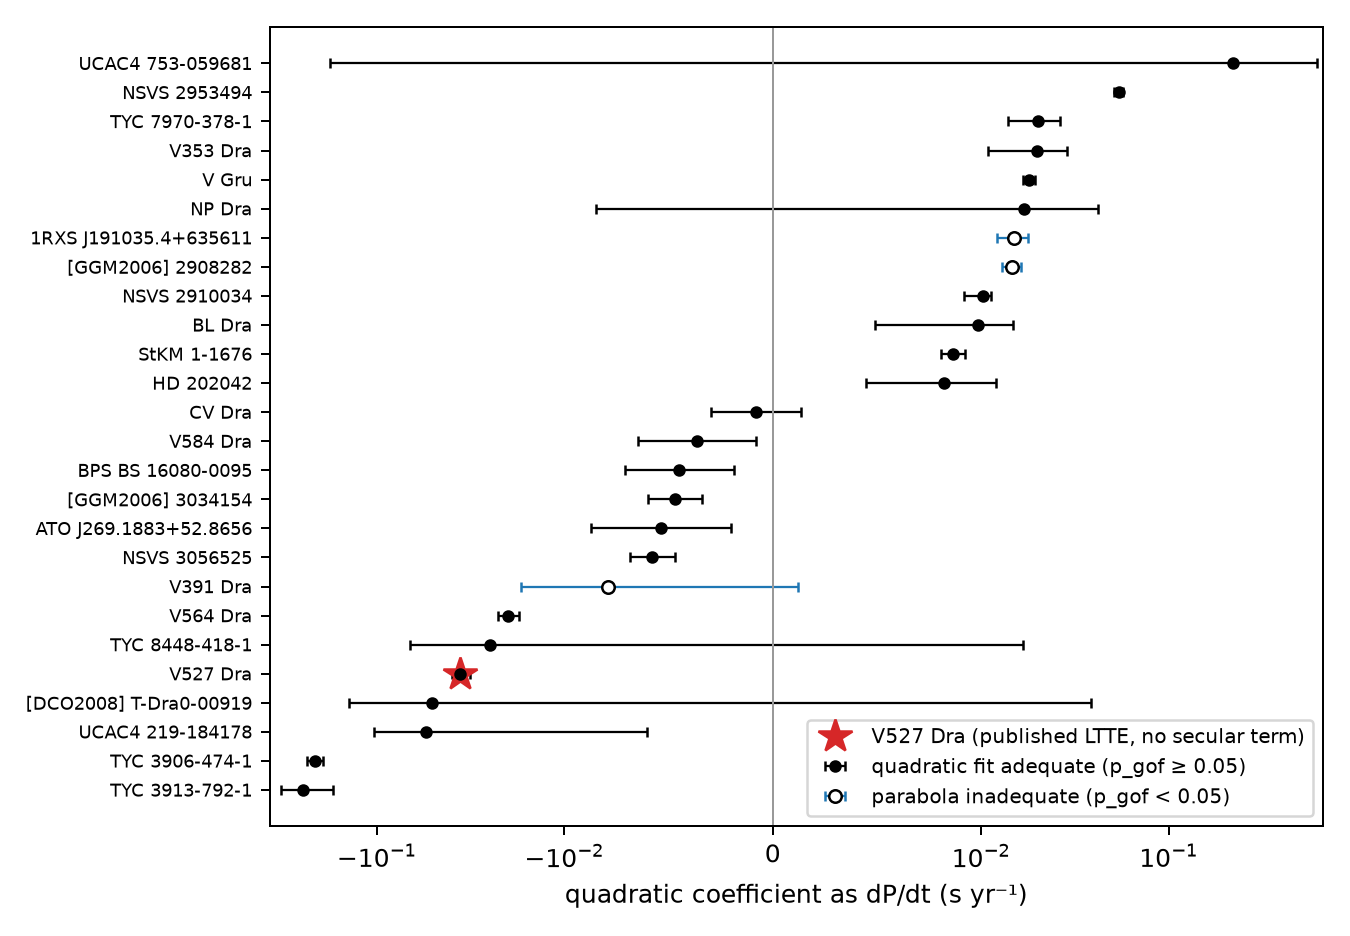
\includegraphics[width=\linewidth]{figures/fig4_dpdt.png}
\caption{Quadratic coefficients $\mathrm{d}P/\mathrm{d}t$ of the 26 targets with 1$\sigma$ bars, ordered by value; the three flagged targets ($p_{\rm gof}$ < 0.05) are shown open, and V527 Dra is marked.}
\label{f:dpdt}
\end{figure}
\begin{sidewaystable*}
\caption{Quadratic ephemerides of the 26 measured targets. Name is the variable-star designation where one exists, otherwise the SIMBAD identifier; positions are those of the TIC (J2000, degrees); $T$ is the TESS magnitude; $P$ the catalogue period in days; $N$ the number of epochs; $\nu=N-3$; span the baseline in years; d$P$/d$t$ the quadratic coefficient expressed as a rate, in s\,yr$^{-1}$. Class: C, curvature surviving the adversarial test; --, none; a, fails the adversarial test; $\dagger$, parabola inadequate ($p_{\rm gof}<0.05$), the coefficient then being that of a model that does not describe the data and listed for completeness only. No entry of this table is a period-change rate: each is a quadratic coefficient over 16--20\,yr, and Sect.~\ref{s:val} shows what such a coefficient can be made of; the table is not to be cited as measured d$P$/d$t$ (Sect.~\ref{s:claim}). V527 Dra (TIC 424461577) passes all three tests and has a published cyclic O$-$C (Sect.~\ref{ss:orb}).}
\label{t:coef}
\centering
\tiny
\begin{tabular}{l l r r r r c c r r r r r r c r}
\hline\hline
TIC & Name & RA & Dec & $T$ & $P$ & $N$ & $\nu$ & span & d$P$/d$t$ & $\chi^2_{\rm red}$ & $p_{\rm gof}$ & $p_{\rm curv}$ & $p_{\rm adv}$ & cl. & blk\\
\hline
115244268 & TYC 7970-378-1 & 317.6428 & -40.5239 & 10.9 & 2.0089 & 5 (3+2) & 2 & 19.9 & +0.0174 $\pm$ 0.0055 & 0.70 & 0.499 & 0.001 & 0.312 & --a & ---\\
126763885 & UCAC4\,219-184178 & 316.2145 & -46.3262 & 12.4 & 4.3574 & 4 (2+2) & 1 & 19.9 & -0.0501 $\pm$ 0.0422 & 1.20 & 0.273 & 0.234 & 0.623 & -- & ---\\
126945917 & HD 202042 & 318.7324 & -43.3954 & 9.1 & 1.3411 & 6 (4+2) & 3 & 19.9 & +0.0099 $\pm$ 0.0035 & 0.53 & 0.664 & 0.004 & 0.665 & --a & ---\\
139256217 & TYC 8448-418-1 & 347.1903 & -46.1102 & 11.0 & 2.1992 & 4 (2+2) & 1 & 19.9 & -0.0274 $\pm$ 0.0408 & 1.07 & 0.300 & 0.501 & 0.861 & -- & ---\\
144194304 & V Gru & 327.9727 & -42.3732 & 9.2 & 0.4835 & 5 (2+3) & 2 & 19.9 & +0.0173 $\pm$ 0.0014 & 0.53 & 0.589 & $<10^{-3}$ & $<10^{-3}$ & C & 7\\
198388252 & [GGM2006] 2908282 & 258.1953 & +57.0529 & 11.6 & 0.3952 & 7 (4+3) & 4 & 19.6 & +0.0141 $\pm$ 0.0016 & 7.66 & $<10^{-3}$ & $<10^{-3}$ & $<10^{-3}$ & C\,$\dagger$ & 7\\
198408416 & NSVS 2910034 & 258.9133 & +58.8645 & 12.1 & 0.3647 & 7 (4+3) & 4 & 19.5 & +0.0099 $\pm$ 0.0011 & 0.64 & 0.631 & $<10^{-3}$ & $<10^{-3}$ & C & 5\\
199688409 & BPS BS 16080-0095 & 253.0515 & +57.7255 & 12.0 & 0.8683 & 7 (4+3) & 4 & 17.6 & -0.0056 $\pm$ 0.0026 & 0.22 & 0.925 & 0.032 & 0.677 & --a & ---\\
207496824 & V353 Dra & 246.9546 & +58.8398 & 10.8 & 0.8027 & 4 (2+2) & 1 & 16.7 & +0.0190 $\pm$ 0.0072 & 2.36 & 0.124 & 0.008 & 0.386 & --a & ---\\
224605072 & [DCO2008] T-Dra0-00919 & 255.5992 & +58.8700 & 11.4 & 0.6649 & 7 (4+3) & 4 & 17.6 & -0.0510 $\pm$ 0.0893 & 0.68 & 0.606 & 0.568 & 0.978 & -- & ---\\
229461186 & BL Dra & 295.1026 & +60.9203 & 10.9 & 0.4027 & 5 (3+2) & 2 & 15.7 & +0.0087 $\pm$ 0.0036 & 0.96 & 0.381 & 0.014 & 0.332 & --a & ---\\
229476285 & UCAC4\,753-059681 & 295.5345 & +60.4830 & 12.9 & 1.0965 & 5 (3+2) & 2 & 15.7 & +0.2189 $\pm$ 0.3975 & 0.79 & 0.455 & 0.582 & 0.762 & -- & ---\\
229687624 & CV Dra & 262.9885 & +57.1784 & 9.0 & 0.6176 & 7 (4+3) & 4 & 19.6 & -0.0013 $\pm$ 0.0021 & 0.56 & 0.691 & 0.542 & 0.686 & -- & ---\\
229914020 & 1RXS J191035.4+635611 & 287.6436 & +63.9373 & 11.9 & 0.6760 & 5 (3+2) & 2 & 15.7 & +0.0133 $\pm$ 0.0023 & 5.42 & 0.004 & $<10^{-3}$ & $<10^{-3}$ & C\,$\dagger$ & 2.5\\
230386284 & StKM 1-1676 & 285.8220 & +63.9928 & 9.0 & 0.3415 & 5 (3+2) & 2 & 15.7 & +0.0081 $\pm$ 0.0006 & 0.07 & 0.928 & $<10^{-3}$ & $<10^{-3}$ & C & 5\\
232634196 & TYC 3906-474-1 & 269.4385 & +56.1960 & 9.9 & 1.2511 & 7 (4+3) & 4 & 19.6 & -0.2181 $\pm$ 0.0207 & 0.72 & 0.578 & $<10^{-3}$ & $<10^{-3}$ & C & $>$ 10\\
237116051 & V391 Dra & 269.7931 & +58.7165 & 10.2 & 2.4629 & 4 (2+2) & 1 & 19.6 & -0.0099 $\pm$ 0.0087 & 13.16 & $<10^{-3}$ & 0.255 & 0.582 & --\,$\dagger$ & ---\\
243352373 & V584 Dra & 290.2686 & +56.3283 & 10.2 & 0.3343 & 4 (2+2) & 1 & 16.7 & -0.0042 $\pm$ 0.0026 & 0.74 & 0.389 & 0.113 & 0.839 & -- & ---\\
329246824 & V564 Dra & 263.8847 & +57.8025 & 11.0 & 0.5877 & 7 (4+3) & 4 & 19.6 & -0.0204 $\pm$ 0.0026 & 0.18 & 0.949 & $<10^{-3}$ & $<10^{-3}$ & C & 7\\
329248002 & NP Dra & 263.8179 & +55.0034 & 8.8 & 3.1089 & 6 (4+2) & 3 & 16.7 & +0.0275 $\pm$ 0.0251 & 0.81 & 0.487 & 0.273 & 0.778 & -- & ---\\
329289186 & ATO J269.1883+52.8656 & 269.1883 & +52.8657 & 13.8 & 0.5525 & 5 (2+3) & 2 & 19.6 & -0.0063 $\pm$ 0.0030 & 0.55 & 0.576 & 0.039 & 0.966 & --a & ---\\
359552377 & TYC 3913-792-1 & 279.3983 & +57.7443 & 10.9 & 3.4391 & 5 (3+2) & 2 & 16.7 & -0.2498 $\pm$ 0.0775 & 0.67 & 0.512 & 0.001 & 0.226 & --a & ---\\
377253090 & NSVS 3056525 & 286.1923 & +58.9513 & 11.8 & 0.4245 & 6 (4+2) & 3 & 16.7 & -0.0061 $\pm$ 0.0010 & 0.52 & 0.670 & $<10^{-3}$ & $<10^{-3}$ & C & 2\\
390021728 & [GGM2006] 3034154 & 277.7934 & +56.4175 & 11.5 & 0.3020 & 6 (4+2) & 3 & 16.6 & -0.0052 $\pm$ 0.0010 & 1.15 & 0.328 & $<10^{-3}$ & 0.004 & C & 2\\
392536812 & NSVS 2953494 & 280.4674 & +58.0565 & 11.2 & 0.5910 & 6 (4+2) & 3 & 16.7 & +0.0536 $\pm$ 0.0029 & 0.24 & 0.866 & $<10^{-3}$ & $<10^{-3}$ & C & $>$ 10\\
424461577 & V527 Dra & 279.7343 & +60.3982 & 10.2 & 0.7448 & 6 (4+2) & 3 & 15.7 & -0.0368 $\pm$ 0.0033 & 2.04 & 0.106 & $<10^{-3}$ & $<10^{-3}$ & C & 10\\
\hline
\end{tabular}
\end{sidewaystable*}
\begin{table*}
\caption{The distribution, in three partitions: all 26 coefficients; the 23 whose quadratic fit is adequate ($p_{\rm gof}\ge0.05$); and the 16 that are adequate and have $\sigma(\mathrm{d}P/\mathrm{d}t)<0.01$\,s\,yr$^{-1}$, a cut on precision rather than on value. No column is a headline: the median $|\mathrm{d}P/\mathrm{d}t|$ moves from 0.009 to 0.018\,s\,yr$^{-1}$ between them, and that sensitivity is the finding.}
\label{t:dist}
\centering
\small
\begin{tabular}{p{0.30\linewidth} p{0.19\linewidth} p{0.20\linewidth} p{0.20\linewidth}}
\hline\hline
Quantity & n = 26 (all) & n = 23 (quadratic fit adequate, $p_{\rm gof}$ $\ge$ 0.05) & n = 16 (adequate and $\sigma(\mathrm{d}P/\mathrm{d}t)$ < 0.01 s\,yr$^{-1}$)\\
\hline
$\mathrm{d}P/\mathrm{d}t$, median & -0.0027 s\,yr$^{-1}$ & -0.0042 s\,yr$^{-1}$ & +0.0034 s\,yr$^{-1}$\\
$|\mathrm{d}P/\mathrm{d}t|$, median & 0.0157 s\,yr$^{-1}$ & 0.0174 s\,yr$^{-1}$ & 0.0093 s\,yr$^{-1}$\\
$\mathrm{d}P/\mathrm{d}t$, interquartile range & [-0.0178, +0.0139] s\,yr$^{-1}$ & [-0.0239, +0.0136] s\,yr$^{-1}$ & [-0.0057, +0.0117] s\,yr$^{-1}$\\
$\mathrm{d}P/\mathrm{d}t$, minimum and maximum & [-0.250, +0.219] s\,yr$^{-1}$ & [-0.250, +0.219] s\,yr$^{-1}$ & [-0.037, +0.054] s\,yr$^{-1}$\\
Sign of $\mathrm{d}P/\mathrm{d}t$: positive / negative (two-sided sign test p) & 12 / 14 (p = 0.85) & 10 / 13 (p = 0.68) & 8 / 8 (p = 1.00)\\
$\sigma(\mathrm{d}P/\mathrm{d}t)$, median & 0.0032 s\,yr$^{-1}$ & 0.0033 s\,yr$^{-1}$ & 0.0026 s\,yr$^{-1}$\\
$\chi^2_{\rm red}$ of quadratic fit, median (25th--75th) & 0.71 (0.53--1.13) & 0.68 (0.53--0.89) & 0.56 (0.45--0.80)\\
$|\mathrm{d}P/\mathrm{d}t|/\sigma$ > 2 / > 3 / > 5 & 18 / 13 / 11 & 16 / 11 / 9 & 14 / 9 / 8\\
Curvature with p < 0.05 & 18 & 16 & 14\\
Curvature surviving the adversarial test & 11 of 26 --- 6 > 0, 5 < 0 & 9 of 23 --- 4 > 0, 5 < 0 & 8 of 16 --- 4 > 0, 4 < 0\\
Same, over targets with detection efficiency $\varepsilon$ > 0 (Sect.~\ref{ss:orb}) & 11 of 24 & 9 of 21 & ---\\
Same, with TESS bars inflated by 1.0 / 2.6 min\,yr$^{-1}$ (Sect.~\ref{ss:setores}, sensitivity ceiling) & 1 / 0 of 26 & 1 / 0 of 23 & 0 / 0 of 16\\
Measured but not tested (d.o.f. < 1) & 0 & 0 & 0\\
$|\mathrm{d}P/\mathrm{d}t|$ > 10 s\,yr$^{-1}$ (cycle-count guard) & 0 & 0 & 0\\
\hline
\end{tabular}
\end{table*}
Five remarks on the table (Fig.~\ref{f:dpdt} shows the coefficients; Fig.~\ref{f:barras} shows what the detections track). (i) In every partition the distribution is consistent with symmetry about zero: 12/14 (sign test p = 0.85), 10/13 (p = 0.68) and 8/8 (p = 1.00). (ii) The median $|\mathrm{d}P/\mathrm{d}t|$ of 0.016 s\,yr$^{-1}$ over all 26 is 1.8 $\times$ $10^{-7}$ d\,yr$^{-1}$, the order of magnitude familiar from period studies of W UMa systems; 0.009 s\,yr$^{-1}$ for the well-measured 16 is 1.0 $\times$ $10^{-7}$ d\,yr$^{-1}$. That median sits just above the amplitude at which the chain's completeness for a secular term is 50\% (0.014 s\,yr$^{-1}$; Sect.~\ref{sss:secular}). The 26 include the non-detections, so the distribution is not truncated, but it is shaped by the sensitivity of the chain at exactly the scale it reports, and the agreement with the W UMa literature --- itself built from chains with their own thresholds --- is not read here as an astrophysical result. (iii) Under the earlier fixed rule $\chi^2_{\rm red}$ $\ge$ 2 the flag would have marked 5 targets instead of 3, and the chance that such a flag lands on one given target by coincidence is then 19\% --- a number that matters in Sect.~\ref{ss:orb}. (iv) Of the 18 targets with $p_{\rm curv}$ < 0.05, seven fail the adversarial gate (TIC 115244268, 126945917, 199688409, 207496824, 229461186, 329289186 and 359552377), and for them the gate, not a look-elsewhere correction, is what excludes them. (v) Two targets (TIC 224605072, 229476285) have no detection sensitivity at the amplitudes considered in Sect.~\ref{ss:orb} ($\varepsilon$ = 0: their SuperWASP bars are too large for the curvature test to reject anything), so their ``no significant curvature'' is not a null result and they do not belong in the count; over the 24 with sensitivity, 11 survive the adversarial test, given as a separate row of Table~\ref{t:dist}.

Two sets are used by name in the rest of the paper. \textbf{D11} is the eleven targets whose curvature survives the adversarial test (TIC 144194304, 198388252, 198408416, 229914020, 230386284, 232634196, 329246824, 377253090, 390021728, 392536812, 424461577); \textbf{D9} is D11 without the two flagged members (198388252, 229914020). One member of D9, TIC 377253090, has an unresolved companion of equal brightness at 1.7\arcsec (CROWDSAP 0.56; Sect.~\ref{ss:epocas}) and is carried with that caveat. The completeness of the chain for a secular term, measured by injection with the same estimator (Sect.~\ref{sss:secular}), is 50\% at 0.014 s\,yr$^{-1}$ and, at the tabulated coefficients of the eleven, 0.66--1.00: the eleven are a count, not a rate. The third flagged target, TIC 237116051, has no surviving curvature. For the two flagged members of D11 the reading is \textit{period variation detected without a determined form}; for the third, \textit{not described by a quadratic ephemeris}; in neither case should the tabulated coefficient be quoted as a rate. Sect.~\ref{sss:teto} applies the measured noise model of the between-sector scale to this design and leaves 7 of the 11; Sect.~\ref{ss:externo} confronts the coefficients of D9 with the complete TESS block of the same targets. The sets have changed with the bars, and Appendix~\ref{a:C} keeps the record.

\begin{table*}
\caption{The window test and the sensitivity to the archival bias, per target. For the nine members of D9, every column of a row comes from the same noise model: the quadratic coefficient of the complete TESS block and its bar under the \textit{least favourable admitted} model --- the admitted model with the largest $\sigma$, which is also the one that sets MDD --- the number of sectors N, the range of z against the tabulated coefficient over all models admitted for that target (Sect.~\ref{sss:teto}), the resulting class (Sect.~\ref{ss:externo}), and \textbf{MDD = 3$\sigma$ of the block coefficient under that same least favourable admitted model}, the smallest difference the block could have shown at 3$\sigma$. The next column gives the pooled-GP fit of the same block, which is \textit{not admitted in any of the eight} (its $\chi^2/\nu$ runs from 0.05 to 6.37, given in brackets): it is kept because it is the only variant comparable across targets, and it is labelled rather than mixed into the columns that carry the classification. V527 Dra is held out of the classification and carries its published light-travel-time orbit instead; its complete fit including the archival seasons is compatible with zero (Sect.~\ref{ss:orb}). The last column, given for all 26, is the change of the tabulated coefficient of Table~\ref{t:coef} per 2.14 min of archival bias (Sect.~\ref{ss:vies}) --- the bias is a first-order term in the value and a zeroth-order term in the verdict.}
\label{t:janela}
\centering
\scriptsize
\begin{tabular}{r l r r r l r r r}
\hline\hline
TIC & Name & block, admitted (s yr$^{-1}$) & N & z (adm.) & class & MDD & pooled GP (s yr$^{-1}$, $\chi^2/\nu$) & $\Delta$ per 2.14 min\\
\hline
115244268 & TYC 7970-378-1 & --- & --- & --- & not in D9 & --- & --- & 0.0053\\
126763885 & UCAC4\,219-184178 & --- & --- & --- & not in D9 & --- & --- & 0.0117\\
126945917 & HD 202042 & --- & --- & --- & not in D9 & --- & --- & 0.0036\\
139256217 & TYC 8448-418-1 & --- & --- & --- & not in D9 & --- & --- & 0.0059\\
144194304 & V Gru & --- & 4 & --- & not testable & --- & --- & 0.0013\\
198388252 & [GGM2006] 2908282 & --- & --- & --- & not in D9 & --- & --- & 0.0011\\
198408416 & NSVS 2910034 & +0.0468 $\pm$ 0.0107 & 39 & +3.4 to +6.1 & contradicted & 0.0321 & +0.0452 $\pm$ 0.0120 (0.33) & 0.0011\\
199688409 & BPS BS 16080-0095 & --- & --- & --- & not in D9 & --- & --- & 0.0030\\
207496824 & V353 Dra & --- & --- & --- & not in D9 & --- & --- & 0.0028\\
224605072 & [DCO2008] T-Dra0-00919 & --- & --- & --- & not in D9 & --- & --- & 0.0020\\
229461186 & BL Dra & --- & --- & --- & not in D9 & --- & --- & 0.0016\\
229476285 & UCAC4\,753-059681 & --- & --- & --- & not in D9 & --- & --- & 0.0026\\
229687624 & CV Dra & --- & --- & --- & not in D9 & --- & --- & 0.0017\\
229914020 & 1RXS J191035.4+635611 & --- & --- & --- & not in D9 & --- & --- & 0.0026\\
230386284 & StKM 1-1676 & +0.0091 $\pm$ 0.0008 & 38 & +1.0 & not contradicted & 0.0024 & +0.0088 $\pm$ 0.0110 (0.05) & 0.0013\\
232634196 & TYC 3906-474-1 & -0.6485 $\pm$ 0.1328 & 43 & -9.5 to -3.2 & contradicted & 0.3983 & -0.7022 $\pm$ 0.0473 (2.16) & 0.0036\\
237116051 & V391 Dra & --- & --- & --- & not in D9 & --- & --- & 0.0057\\
243352373 & V584 Dra & --- & --- & --- & not in D9 & --- & --- & 0.0012\\
329246824 & V564 Dra & -0.0001 $\pm$ 0.0066 & 42 & +2.9 & ambiguous & 0.0197 & -0.0036 $\pm$ 0.0196 (0.30) & 0.0017\\
329248002 & NP Dra & --- & --- & --- & not in D9 & --- & --- & 0.0111\\
329289186 & ATO J269.1883+52.8656 & --- & --- & --- & not in D9 & --- & --- & 0.0016\\
359552377 & TYC 3913-792-1 & --- & --- & --- & not in D9 & --- & --- & 0.0123\\
377253090 & NSVS 3056525 & -0.0050 $\pm$ 0.0049 & 40 & -0.0 to +0.2 & not contradicted & 0.0146 & -0.0022 $\pm$ 0.0139 (0.56) & 0.0015\\
390021728 & [GGM2006] 3034154 & +0.0286 $\pm$ 0.0088 & 41 & +3.8 to +5.5 & contradicted & 0.0263 & +0.0272 $\pm$ 0.0103 (1.98) & 0.0011\\
392536812 & NSVS 2953494 & +0.0209 $\pm$ 0.0074 & 42 & -4.1 & contradicted & 0.0223 & +0.0184 $\pm$ 0.0216 (0.45) & 0.0021\\
424461577 & V527 Dra & -0.0090 $\pm$ 0.0564 & 40 & --- & published LTTE & --- & +0.0513 $\pm$ 0.0264 (6.37) & 0.0029\\
\hline
\end{tabular}
\end{table*}


\section{Three mechanisms that can produce a period change, and what the data can test}\label{s:val}
\begin{figure*}
\centering
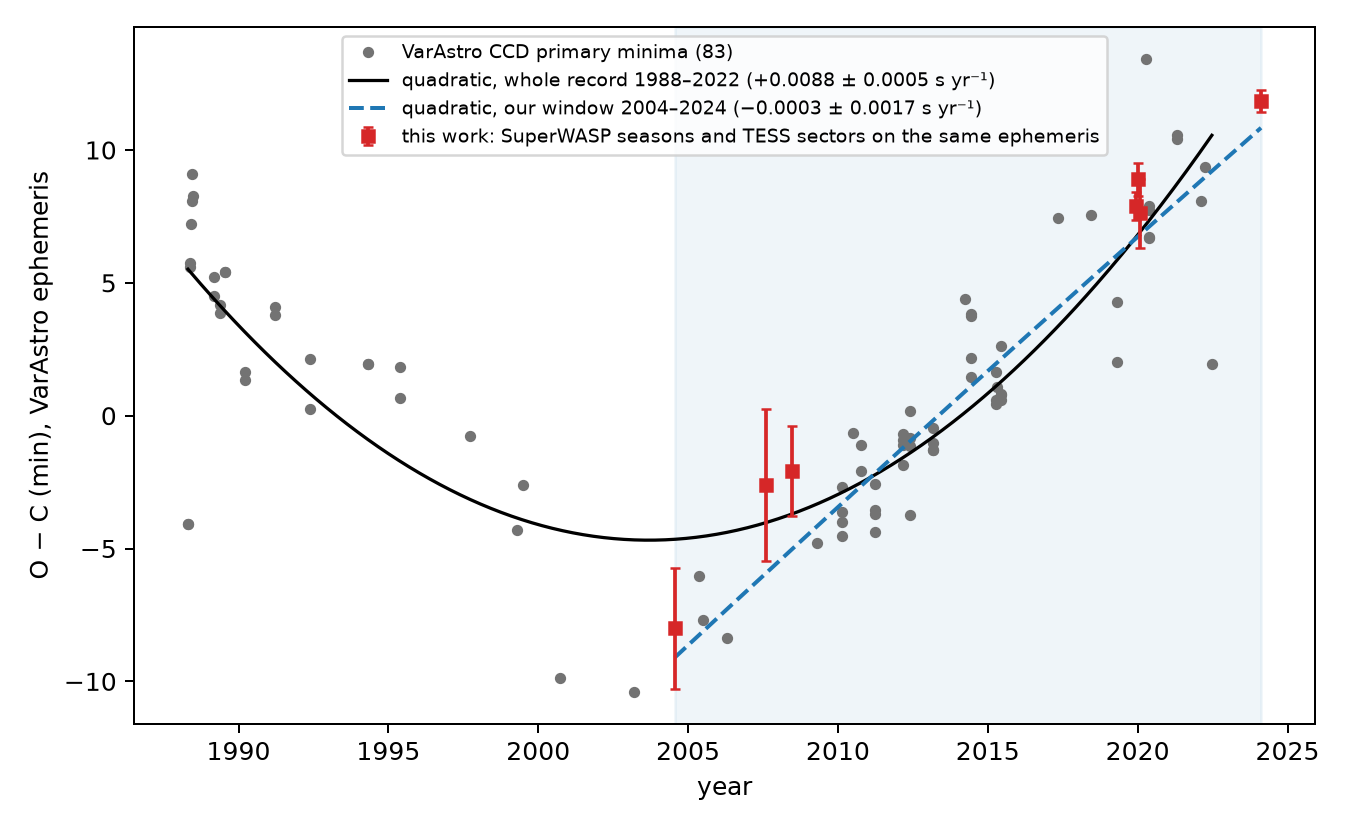
\includegraphics[width=\linewidth]{figures/fig3_cvdra.png}
\caption{CV Dra: VarAstro CCD primary minima 1988--2022 with the quadratic fitted to the whole record and the one fitted to our 2004--2024 window, and our epochs placed on the same ephemeris.}
\label{f:cvdra}
\end{figure*}
Each mechanism is stated, quantified on the 26, and confronted with what the data can and cannot test. The demonstration that frames all three is external and independent of the cache: for CV Dra, the one target with 34 years of independent CCD minima, a quadratic fitted to the same 2004--2024 window reproduces our coefficient (4 of 4 agree), and a quadratic fitted to the whole record does not (2 of 5; Fig.~\ref{f:cvdra}; Sect.~\ref{ss:externo}). The object called ``$\mathrm{d}P/\mathrm{d}t$ over 16--20 yr'' is a local coefficient of a curve that is not polynomial; the three mechanisms below are the ways such a coefficient acquires a significance it does not have. The control target (TIC 142874476), on which the chain was developed, was re-run before and after every change reported in this version and reproduced each time; its record and the period-ladder audit are internal quality assurance and are given in Appendix~\ref{a:A}.


\subsection{Formal timing errors}\label{ss:formais}
\textbf{Formal errors against the residuals.} The reduced $\chi^2$ of the quadratic fit is the check that the assigned errors describe the residuals. With formal errors it had median 6.35 (25th--75th: 2.08--37.5), was below 2 for only 8 of 31, and left maximum quadratic residuals of 4.4 min (median) to 18 min (75th percentile) against bars of 0.4--0.7 min: not even the more complex model explained the residuals, which locates the problem in the denominator, not the model.

\textbf{Consequence of the formal-error run.} That run --- kept in full as \texttt{oc\_\allowbreak lote\_\allowbreak barras\_\allowbreak formais/} --- returned 24 of 31 targets with $|\mathrm{d}P/\mathrm{d}t|/\sigma$ > 3 and 23 surviving the adversarial test. The comparison that matters is on the same targets: over the 26 that the data-derived chain measures, the formal bars give 20 with $|\mathrm{d}P/\mathrm{d}t|/\sigma$ > 3 and 19 surviving the adversarial gate, against 13 and 11 with the bars of Sect.~\ref{ss:barras} --- the same designs, the same estimator, only the denominator changed. The 13-sigma ``detection'' that headed the formal-error list (TIC 199688472, +1.75 $\pm$ 0.006 s\,yr$^{-1}$) was a quadratic bending to reach two SuperWASP seasons of $\pm$76 min at 19 yr of leverage, one of which had a negative fitted depth; the target is now in Table~\ref{t:naomedidos}, and the entire positive tail of that distribution (95th percentile +0.84 s\,yr$^{-1}$, now a maximum of +0.22) consisted of such targets. Formal timing errors in archival photometry produce spurious period changes in bulk, and they produce them preferentially with large leverage, where they look most significant.


\subsection{The residual test and its null: what data-derived bars can be validated against}\label{ss:qualbarra}
\begin{figure*}
\centering
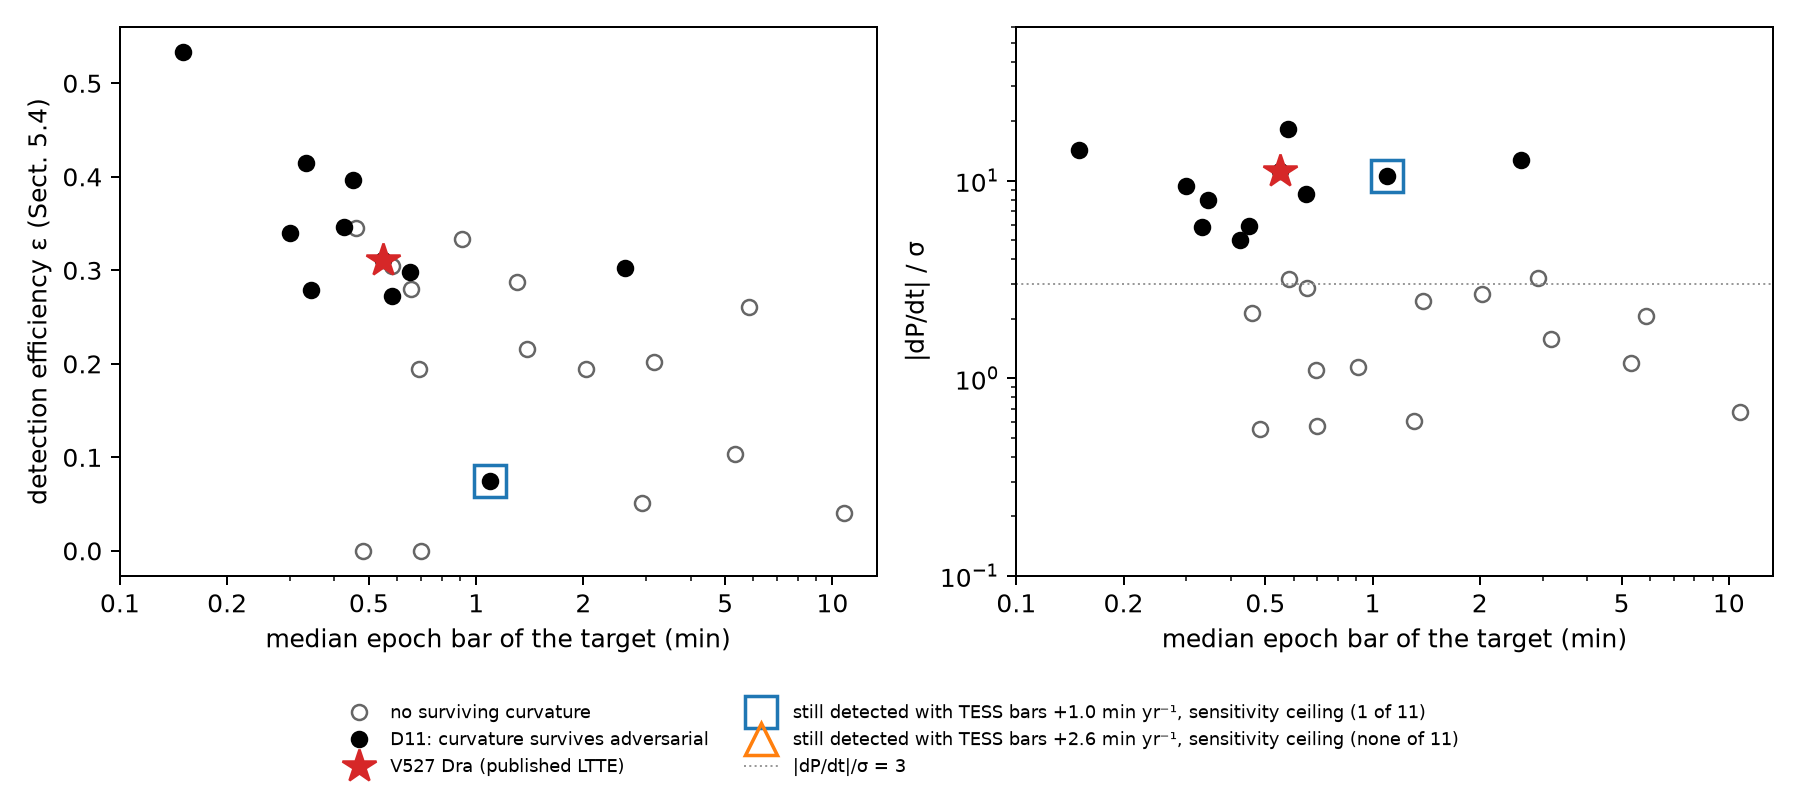
\includegraphics[width=\linewidth]{figures/fig1_barras.png}
\caption{Detection efficiency, significance and the bars. Left: the per-target detection efficiency $\varepsilon$ of Sect.~\ref{ss:orb} against the median epoch bar of the target; right: $|\mathrm{d}P/\mathrm{d}t|/\sigma$ against the same bar. Filled symbols are D11 and the star is V527 Dra; the open squares and triangles mark the targets still detected under the \textit{ceiling} of Sect.~\ref{sss:teto}, with the TESS bars inflated by 1.0 and 2.6 min\,yr$^{-1}$ (one target and none) --- not under the admitted noise model of record, which leaves seven (Table~\ref{t:janela} gives the window test of each). The dotted line in the right panel is $|\mathrm{d}P/\mathrm{d}t|/\sigma$ = 3.}
\label{f:barras}
\end{figure*}
This subsection is about the test that validates data-derived bars --- the residuals of the quadratic fits, normalised by the bar of each epoch, corrected for leverage and summed by data set --- and its result is a property of the test rather than of the sample. Stated first: when each bar is estimated from the same two or three samples that enter the residual, the null of the test is \textbf{0.77 and not 1}, so a reduced $\chi^2$ near 0.7 is what correct bars \textit{produce} in this design. Against that null the bars of Sect.~\ref{ss:barras} are consistent with the residuals of the 26 except in three targets whose quadratic the goodness-of-fit test rejects, which hold the excess of both archives; over the other 23 both archives are inside their nulls once the same cut is applied inside the simulation. The reading is narrower than ``the bars are right'', because the test cannot separate correct bars from bars inflated by real secular terms of the tabulated size. The path to this result passed through an archival excess of 2.73 that three tests treated as real --- a composition error of 1.74 in the bars, and the remainder measured against a null of 1 --- and the readings built on it are withdrawn (Appendix~\ref{a:C}); the simulations and their committed expectations are in Appendix~\ref{a:D}.


\subsubsection{The data-derived bars against the expected reduced \texorpdfstring{$\chi^2$}{chi2}}\label{sss:esperado}
With errors from the data (Sect.~\ref{ss:barras}) the median reduced $\chi^2$ of the 26 quadratic fits is 0.71. With 1--4 degrees of freedom the median of $\chi^2/\nu$ under correct bars is well below 1, and for the actual distribution of degrees of freedom of the 26 the expected median is 0.73 (95\% range 0.43--1.15; 20\,000 simulations); 0.71 has probability 0.56 of being this high. The aggregate does not: reduced $\chi^2$ 1.44 over 67 degrees of freedom, of which the three targets the goodness-of-fit test rejects contribute more than half, the other 23 giving 0.70. Both comparisons assume the bars are known; they are not, and Sect.~\ref{sss:nulo} simulates the null of the pipeline's own estimator. Against that null the median reduced $\chi^2$ is 0.74 (2.5--97.5\%: 0.54--0.96) and the measured 0.71 sits at its 39th percentile; the aggregate null is 0.90 (0.65--1.26) and the measured 1.44 is above all but 15 of its 2\,000 realisations --- an excess, which the decomposition of the next two subsections locates in the three flagged targets: without them the aggregate of the 23 is inside the null. Earlier versions measured different values here and built a bar correction on them; the difference is the composition error of the next subsection, and those readings are withdrawn (Appendix~\ref{a:C}).


\subsubsection{The leverage-corrected decomposition by data set, and the composition error it exposed}\label{sss:decomp}
A global $\chi^2$ says whether the total variance is described, not where a problem sits. The residuals of the quadratic fits, normalised by the bar of each epoch and corrected for leverage --- with three parameters on 4--7 points, $E[r^2/\sigma^2]=1-h$, and h reaches 0.6 for the TESS epochs --- were summed separately over the 84 TESS and 61 SuperWASP epochs of the 26 targets (\texttt{src/\allowbreak qual\_\allowbreak barra\_\allowbreak 26.py}; expectation written before running: excess in TESS). The SuperWASP epochs give $\Sigma z^2$ = 46.5 against 35.4 expected under known bars, a variance factor of 1.31 ($\chi^2$ interval 0.87--2.23; bootstrap over targets 0.62--2.30); the TESS epochs give 50.2 against 31.6, a factor of 1.59 (1.02--2.79; 0.54--3.08). The mean leverage is 0.62 for the TESS epochs and 0.42 for the SuperWASP ones: the test retains 38\% of the TESS variance and 58\% of the SuperWASP variance. Under the TESS bar of the previous version (Sect.~\ref{ss:barras}) the TESS factor was 1.02 (0.66--1.79): the $\sqrt{2}$ in the bar hid a factor of 1.5 in the TESS residuals, and where that factor sits is located below.

These are not the numbers the first decomposition returned: it gave a SuperWASP factor of 2.73, read as bars 1.65 times too small, because the routine that measures the between-season dispersion returned the standard error of the season \textit{mean} and the batch chain needs the dispersion itself --- a factor of 1.74 in variance, at the seam between two callers of one function, where the control target could not see it. The correction, what it moved and the version built on the earlier number are in Appendix~\ref{a:C}.

The test is asymmetric: it has power for SuperWASP, whose epochs sit at the end of the lever, and little for TESS, whose four epochs are fitted by three parameters --- what the parabola absorbs does not appear as a residual. A TESS excess at the between-sector scale is therefore not excluded by this test, only not required by it. The estimator itself is unbiased when the bars are known, and a coherent structure at the TESS epochs raises the TESS factor first --- which is how the measured 1.59 bounds such structure at about 2.5 min (Appendix~\ref{a:D}). What the test cannot see is structure \textit{inside} the parabola --- a drift linear or quadratic over four epochs is absorbed into the coefficient --- and that is the blindness that matters, because it is exactly the between-sector drift of Sect.~\ref{ss:setores}.


\subsubsection{The null of the estimator: bars re-estimated from two or three samples}\label{sss:nulo}
The $\chi^2$ interval quoted above assumes the bars are known. They are not: each SuperWASP bar is the standard deviation of 2--3 season deviations that also enter the residual, and each TESS bar is max(formal, $|t_a - t_b|/2$) from the two halves of the sector, so s is estimated from the same points as r and the null has to be simulated as the pipeline operates (\texttt{src/\allowbreak nulo\_\allowbreak barras\_\allowbreak reestimadas\_\allowbreak 26.py}; 2\,000 realisations on the 26 real designs, the setup, the committed expectation and the grids in Appendix~\ref{a:D}).

With the bars re-estimated, the null of the SuperWASP factor is \textbf{0.77} (2.5--97.5\%: 0.63--0.94) and the TESS null 0.98. What deflates it is not the small number of degrees of freedom but the \textbf{floors}: the bar is the larger of the co-estimated dispersion and the formal error and carries the bias term in quadrature, so whenever the dispersion of two or three samples falls below a floor the bar exceeds it while the residual does not --- remove the floors in the simulation and the null returns above 1 (Appendix~\ref{a:D}). The control is the same simulation with the bars held \textbf{fixed}, which returns \textbf{1.00} in both sets: the estimator is unbiased when $\sigma$ is known and biased low when $\sigma$ is co-estimated, and the second case is the pipeline. A reduced $\chi^2$ near 0.7 is therefore what correct bars \textit{produce} in this design, and it is the number to compare with rather than a sign of over-estimated bars.

Against its own null the measured SuperWASP factor of 1.31 is not a small-$\nu$ artefact but an excess: none of the 2\,000 realisations reaches it. The measured TESS factor of 1.59 sits at the 94th percentile of its null --- a milder excess, on the side the test has least power for. Where it sits is a reading made after the fact and labelled as such, but the criterion it uses is the one Sect.~\ref{ss:testes} declares, not one chosen after seeing the residuals: the three targets whose quadratic the goodness-of-fit test rejects ($p_{\rm gof}$ < 0.05; TIC 198388252, 229914020, 237116051) contribute more than half of the 46.5 on the SuperWASP side, and 19.6 (198388252) and 10.7 (229914020) of the 50.2 on the TESS side. Over the 23 targets with an adequate quadratic the SuperWASP factor is 0.72 and the TESS factor 0.68, each at the 24th percentile of a null simulated with the \textit{same} goodness-of-fit cut applied inside every realisation --- the conditioning matters, and how it was done is in Appendix~\ref{a:D}. The excess is not in the bars of either archive; it is in three targets whose parabola does not describe the data, and one of them, TIC 198388252, is a member of D11 --- a detection that passes the significance and adversarial tests on a quadratic the goodness-of-fit test rejects, the same structure as V527 Dra with a different confounder (Sect.~\ref{ss:orb}). No bar correction is applied: the bars of Sect.~\ref{ss:barras}, with the composition error corrected, are the bars of Tables~\ref{t:coef}--\ref{t:janela}, and the earlier ``corrected'' and ``jointly corrected'' sets of detections are withdrawn (Appendix~\ref{a:C}).

\textbf{What the test cannot separate.} A real secular term inflates the co-estimated archival bar (Sect.~\ref{sss:secular}), and an inflated bar lowers the factor, so a sample whose bars are right and a sample carrying real terms of the tabulated size give the same reading. Injecting a term in every target and re-measuring (\texttt{src/\allowbreak completude\_\allowbreak secular\_\allowbreak 26.py --fator}) makes the archival factor fall monotonically with the amplitude while the TESS factor stays put, and the measured 0.72 of the 23 is as likely under no term as under 0.01--0.02 s\,yr$^{-1}$ in every target; what the test does exclude is a term of 0.05 s\,yr$^{-1}$ in every target. The mechanism is the coupling between bar and residual, not a migration of the fit to the TESS block --- the leverage of the archival epochs does not move --- and the grids of both are in Appendix~\ref{a:D}. \textbf{What this subsection can say is therefore narrower than ``the bars are right'': the bars are consistent with the residuals, and so would be bars inflated by real terms of up to about 0.02 s\,yr$^{-1}$ in every target.}


\subsubsection{What the residuals leave for orbits, with the same estimator}\label{sss:orbitas}
An undersampled third-body orbit is the structure that the four TESS epochs absorb into the parabola and the SuperWASP seasons, 12--16 yr away, do not. How much of an archival excess such orbits could produce was measured by injecting the declared population of Sect.~\ref{ss:orb} into the 26 designs with occurrence f, \textbf{with the bars re-estimated inside the simulation}, and reading the two factors (\texttt{src/\allowbreak estrutura\_\allowbreak swasp\_\allowbreak 26.py}; the first run held the bars fixed, whose null is 1.00 against the measurement's 0.77, and the numbers it gave are withdrawn as cross-estimator comparisons --- Appendix~\ref{a:C}). Two results, with the grid in Appendix~\ref{a:D}: the re-estimated bars absorb most of an orbit's between-season signal, so \textbf{the archival side is nearly blind to orbits} and the TESS side is where they would show; and the archival excess of the three flagged targets is not an orbit population, since even at an occurrence of one the probability that orbits alone produce the measured SuperWASP factor is 0.16. The TESS side places no useful bound on the tertiary fraction: nothing below the highest published value is excluded, and the central value is taken from Tokovinin et al. and not from here.


\subsubsection{A secular term through the same estimator: completeness and self-suppression}\label{sss:secular}
The two subsections above ask what the estimator does to noise and to orbits; this one asks what it does to the signal the paper is nominally about. A pure secular term was injected on the 26 real designs at $|\mathrm{d}P/\mathrm{d}t|$ = 0.005--0.25 s\,yr$^{-1}$ (the median tabulated $|\mathrm{d}P/\mathrm{d}t|$ is 0.016), with the bars re-estimated inside each realisation by the pipeline's rule --- for SuperWASP the dispersion of the simulated seasons \textit{with the signal in them}, because a real secular term appears as season-to-season spread --- and each realisation judged by the curvature test and the adversarial gate (\texttt{src/\allowbreak completude\_\allowbreak secular\_\allowbreak 26.py}; the full setup and the two committed expectations are in Appendix~\ref{a:D}). Fig.~\ref{f:compl} shows the two curves of every target.

\textit{Completeness.} With no term injected the gate fires in 0.0\% of realisations at the median target and in at most 6\% in 23 of the 26; summed over the 26 the false-alarm rates give 0.39 detections expected from noise alone, and no member of D11 has a rate above 1.0\%. The amplitude at which half the injected terms are detected has a median of 0.014 s\,yr$^{-1}$ --- the median tabulated coefficient is 0.016 --- and completeness at 0.02 s\,yr$^{-1}$ is $\ge$ 0.5 in 16 of the 26; at 0.2 s\,yr$^{-1}$ it exceeds 0.9 in 21 and stays below 0.75 in the three targets with archival bars above 15 min, which are also the three that never reach 0.5 on the grid. At the coefficient each of them carries in Table~\ref{t:coef}, the eleven members of D11 have a completeness of 0.66--1.00 (median 0.93): the denominator of ``eleven detections'' is not eleven, and no count of detections in this paper is a rate. What sets the 50\% amplitude, and what re-estimating the bars costs in completeness, are in Appendix~\ref{a:D}.

\textit{Self-suppression.} The re-estimated bars contain the signal, and the signal inflates them. Against the expectation of a 20--40\% effect at 0.2 s\,yr$^{-1}$, $\sigma(\mathrm{d}P/\mathrm{d}t)$ with re-estimated bars exceeds $\sigma$ with the true bars by a median factor of 1.03 at 0.02 s\,yr$^{-1}$, 1.19 at 0.05, 1.6 at 0.1 and 2.9 at 0.2 --- and by 5--24 at 0.2 in the 9 targets whose archival seasons have bars of 1.5--5 min at the longest lever (up to $\times$24). The simulated noise is the assigned bar of each epoch, which on a target with real structure already contains it, so the suppression measured is a floor. The reason for it is arithmetic: a term of 0.02 s\,yr$^{-1}$ at E $\approx$ $-$8000 cycles moves two seasons 730 cycles apart by about 3 min relative to each other, the size of the bars; at 0.2 s\,yr$^{-1}$ the between-season spread of the signal is tens of minutes and the ``bar'' is made of it. The coefficient itself is unbiased (median recovered/injected 1.00--1.01) and the goodness-of-fit cut does not see the term: the estimator cannot manufacture a detection from a secular term, but it turns the tabulated $\sigma$ of a real one into an overestimate that grows with the term, and it hides real terms near the 50\% point. This is an estimator property of the same family as the composition error of Sect.~\ref{sss:decomp} --- each season's bar estimated from the seasons themselves --- and, unlike it, not corrected here; the alternatives that would break the coupling, none implemented in this version, are listed in Appendix~\ref{a:D}. For TIC 232634196 the simulation on its own design, with the noise taken as its 19.9-min bars, gives a completeness of 0.94 and a suppression of 1.7 at its coefficient; if those bars were instead the signal's own spread on the 1.4-min formal noise --- which is what the simulation produces for a term of that size on the small-bar designs --- the tabulated $\sigma$ would be an overestimate by an order of magnitude. The data decide against the second reading on one point: if the 19.9 min were the term's own spread on 1.4-min formal noise, the three seasons would fall on the fitted parabola within about 1.4 min, and they fall at 13, 0 and $-$22 min from it.

\begin{figure}
\centering
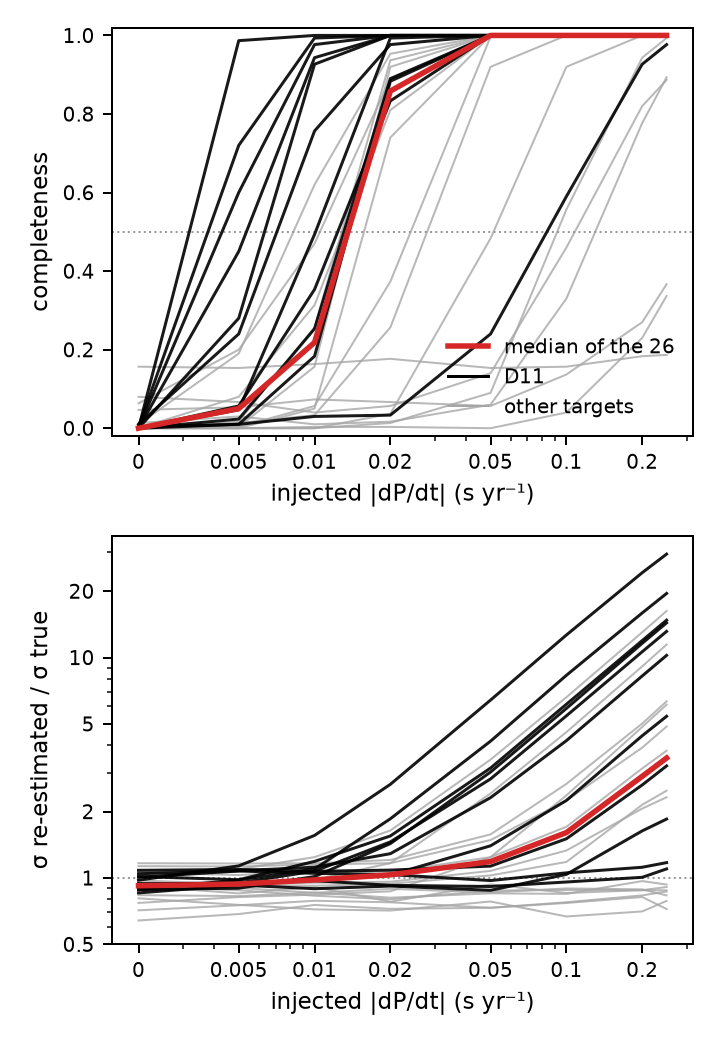
\includegraphics[width=\linewidth]{figures/fig5_completude.png}
\caption{A secular term through the estimator of the chain (Sect.~\ref{sss:secular}). Top: completeness --- the fraction of injected terms passing the curvature test and the adversarial gate with the bars re-estimated inside the simulation --- against the injected $|\mathrm{d}P/\mathrm{d}t|$, one curve per target (black: D11; grey: the others; red: the median of the 26; the point at 0 is the false-alarm rate). Bottom: the suppression factor, $\sigma(\mathrm{d}P/\mathrm{d}t)$ with the re-estimated bars over $\sigma$ with the true bars, on the same grid. Both are properties of the 4--7-epoch design, not of the complete TESS block of Sect.~\ref{ss:externo}.}
\label{f:compl}
\end{figure}

\subsection{Between-sector timing noise: the secondaries and the TESS sensitivity ceiling}\label{ss:setores}

\subsubsection{Secondary minima: the differential drift between sectors}\label{sss:secundarios}
Apsidal motion in an eccentric orbit produces a spurious quadratic in the primary alone, with the secondary moving the opposite way; a secular $\mathrm{d}P/\mathrm{d}t$ moves both together. The secondary epoch was measured in every TESS sector of the 26 with the same estimator, the catalogue seed shifted by P/2, the same trapezoid and the same halves-dispersion bar (\texttt{src/\allowbreak secundarios\_\allowbreak 26.py}; expectation written before running: most secondaries measurable, 0--2 targets with a significant differential drift, up to 5 with no measurable secondary). The quantity tested is d = t\_sec $-$ t\_prim $-$ P/2 per sector, and its drift between the first and last sector (median lever 4.2 yr within TESS).

All 26 secondaries were measurable; for two of the long-period targets (TIC 139256217, 359552377) the bar on d exceeds 10 min and the test is uninformative, leaving 24. In 7 of the 24 the secondary sits more than 2$\sigma$ from phase 0.5 (TIC 126763885, 198388252, 224605072, 229914020, 232634196, 329246824, 329289186), which is a statement about eccentricity or asymmetry, not about period change. In 6 of the 24 the differential drift is significant at > 2$\sigma$ --- more than the 0--2 expected: TIC 115244268 (+1.26 $\pm$ 0.50 min\,yr$^{-1}$), 229476285 ($-$1.50 $\pm$ 0.31), 229914020 (+2.59 $\pm$ 0.25; flagged), 232634196 ($-$1.80 $\pm$ 0.49), 329289186 (+2.41 $\pm$ 0.42), 390021728 (+0.67 $\pm$ 0.24) (under the TESS bar of the previous version the sixth, TIC 115244268, was at 1.9$\sigma$ and five were significant). One of the four targets with P > 2 d and an informative secondary shows a drift (TIC 115244268, P = 2.01 d, at 2.5$\sigma$), so the eccentric-orbit confounder is not excluded where it was expected; the other five drifts occur in systems with P = 0.3--1.25 d, where migrating spots are the usual cause of differential primary/secondary timing (Tran et al. 2013; the displacement of the light centroid that produces it is worked out in Kalimeris et al. 2002).

Of the eleven detections of D11, three are affected. TIC 229914020 has the largest differential drift of the sample (+2.59 $\pm$ 0.25 min\,yr$^{-1}$, 10$\sigma$), is flagged by the goodness-of-fit test, and is in D11: its curvature, its bad fit and its drifting secondary are three views of the same non-quadratic timing behaviour, and the target belongs to none of the categories that read as period change. TIC 232634196 has a differential drift of $-$1.8 $\pm$ 0.5 min\,yr$^{-1}$ over 4.2 yr, which extrapolated over the 20-yr baseline --- an illustration, since it was measured on a fifth of it --- would be 36 min against a quadratic excursion of 201 min, so the secondary shares part of that curvature and not necessarily all of it. TIC 390021728 has the smallest of the six drifts (+0.67 $\pm$ 0.24 min\,yr$^{-1}$), which extrapolated the same way is 13 min against a quadratic excursion of 13 min: its curvature and its secondary's drift are of the same order. The primary/secondary test qualifies three of the eleven; it does not bear on the third-body mechanism of Sect.~\ref{ss:orb}, which moves both minima together.

The excess itself --- six drifts against 0--2 expected --- is the measurement that motivates the next subsection: a drift of 0.7--2.6 min\,yr$^{-1}$ between sectors years apart is invisible to a within-sector bar and to the residual test. Whether the primaries drift as the secondaries do is no longer left open here: the 799 cached sectors measure it directly.

\textbf{The mean and the difference, over the complete block.} Migrating spots displace the primary and the secondary in opposite directions --- Tran et al. (2013) find that pattern in the close binaries of the Kepler field, with amplitudes of 200--300 s, Kalimeris et al. (2002) give the mechanism as a displacement of the light centroid, and Balaji et al. (2015) track the spot longitudes that produce it --- while anything that moves the system as a whole, a third body or a secular term, displaces both together. Averaging the two minima is therefore the standard way to suppress the spot component (Borkovits et al. 2016), and the cached sectors allow it directly: M = (O$-$C\_p + O$-$C\_s)/2 and D = O$-$C\_p $-$ O$-$C\_s, grouped by calendar year as in Sect.~\ref{ss:externo} (\texttt{src/\allowbreak media\_\allowbreak diferenca\_\allowbreak oc\_\allowbreak d9.py}; 22 targets with at least 20 sectors in both minima, plus HD 202042). The asymmetry of the test is stated before its result: the mean cancels \textit{only} the anticorrelated component, and spots that are polar, or persistent over the hemisphere that is not eclipsed, displace both minima the same way and survive it. ``It is in the difference, therefore there is a spot component'' is sound; ``it is in the mean, therefore it is not spots'' is not, and is not claimed here.

\textbf{What the test finds, and where it fails.} Eight targets carry the test: the seven the window test classifies, and TIC 229914020, a detection whose design fit is flagged (Sect.~\ref{s:res}). That membership was fixed in the expectation written and committed before the measurement, and it does not follow a rule: TIC 198388252 is a detection with a flagged fit and the same 39 sectors, and it is outside the set. The mismatch between the set and any rule that would generate it was found after the measurement, with the value of the excluded target already in hand, so re-drawing the set here would be choosing it with the survivor in view; it is left as declared. The rule one would write instead --- detections with both minima in the complete block, minus the held-out target --- gives nine targets, and what it returns is reported in full in Appendix~\ref{a:D}. Among them the anticorrelated component appears in \textbf{one}: TIC 377253090 (per-sector correlation between the two O$-$C series r = -0.36, p = 0.02). In \textbf{6} the correlation is positive (+0.07 to +0.80): the two minima move together. The eighth, TIC 390021728, sits at the boundary with r = -0.31 (p = 0.050) and is counted in neither group. Two criteria are given because the second was written after the first had been run --- the same order Sect.~\ref{sss:teto} declares for its admission criterion, and it is stated here for the same reason. The criterion written before the run, an annual r < 0 together with a difference series that rejects a constant at 5\%, selects TIC 199688409, 329289186 and 377253090; the one written after, a per-sector r < 0 with p < 0.05, selects TIC 126945917, 237116051 and 377253090. Only TIC 377253090 is in both --- the target with an unresolved companion of nearly equal brightness at 1.7\arcsec (Sect.~\ref{ss:epocas}).

\textbf{What the difference series bounds.} A classification is not the useful output of this test; a limit is. If a spot pattern displaces the primary by +$\delta$ and the secondary by $-\delta$, the difference series carries 2$\delta$, so the white excess of that series over its own bars bounds $\delta$ directly. Fitted by maximum likelihood on each target and taken at 95\% (\texttt{src/\allowbreak media\_\allowbreak diferenca\_\allowbreak oc\_\allowbreak d9.py}), and expressed peak-to-peak, the bound on the anticorrelated component runs from 0.26 to 6.38 min over the eight. The model behind it is D = constant + noise + white excess, with no drift term, so a difference series that drifts has that drift inside the excess: fitting a linear term in D as well removes 5--64\% of the 95\% excess in the 5 targets whose difference series drifts, which is the margin by which the published bound is conservative rather than a correction to it.

\textbf{What it is a fraction of.} The bound is only meaningful against the wander it is meant to explain, and that quantity has to be named, because two of them are in this paper. The excursion of the primary's yearly means about a \textbf{linear} ephemeris of the same block carries the block's own secular term: in TIC 232634196, whose block coefficient is the largest of the sample, it is 12.36 min, of which the parabola accounts for most. The excursion about a \textbf{quadratic} fitted to the same block is what no smooth term explains, and it is the quantity a spot pattern would have to produce: over the eight it runs from 0.08 to 5.02 min, and in TIC 232634196 it is 5.02 rather than 12.36. Sect.~\ref{ss:externo} uses a third, the excursion about the quadratic fitted to design \textbf{and} archive, which for the same target is 8.46 min; the three differ by construction and only the second belongs in this ratio.

\textbf{And what the fraction says.} Against that denominator the bound is 63--535\% of the wander: it is below the wander in 2 of the eight (TIC 198408416 and 329246824, at 88\% and 63\%) and above it in the other 6, and in \textbf{none} of them does it fall below half. An earlier version of this section divided by the linear excursion and reported the bound below the wander in five of the eight and below half in two; that was the denominator carrying the secular term, and the reading it supported --- that an anticorrelated spot pattern is excluded as the principal cause in those two --- \textbf{is withdrawn} (Appendix~\ref{a:C}). What the measurement supports is the weaker and still useful statement: the anticorrelated component is bounded, and in six of the eight the bound is too loose to exclude anything. V527 Dra is not one of the eight --- the set excludes it, because it is the target held out of the classification --- and there the picture is different: its bound is 0.49 min peak-to-peak against a wander of 7.33 min about the quadratic and 7.34 about the linear ephemeris --- 7\% either way, because the target has no significant block curvature for the quadratic to remove.

\textbf{Moving together is not the same as moving together quietly.} Two columns separate what one correlation coefficient hides: the sign of r, and whether the difference series drifts. In 4 of the 6 targets with positive r the difference carries a significant drift (TIC 198408416, 229914020, 230386284 and 232634196) --- TIC 198408416 is the clearest, with r = +0.80 and a drift of -0.300 $\pm$ 0.040 min\,yr$^{-1}$ over its 39 sectors. ``The two minima move together'' describes the correlation, not the residual: underneath it there can be a differential drift that the correlation does not see. Three criteria appear in this subsection and they select three different sets, which is a statement about the criteria and not about the targets: an annual r < 0 with a difference series that rejects a constant (3 targets), a per-sector r < 0 with p < 0.05 (3 others), and a significant drift in D (5, of which 4 are among the six with positive r). None of them carries the result. The limit does, and it is independent of all three: it asks how much anticorrelated amplitude fits inside the difference series, whatever the sign of the correlation and whether or not the series drifts --- and the drift, where there is one, is inside the bound.

\textbf{The held-out target, and what it costs.} V527 Dra, held out of the classification throughout this paper, is the only target of the 26 where both signals are known: a published light-travel-time orbit and migrating spots documented in its light curve (Čeki et al. 2024). The test sees the first and not the second. The per-sector correlation is r = +0.98 --- both minima moving together, which is what an orbit requires --- the difference series is consistent with a constant (p = 0.08 over the annual means, amplitude 2.2 min against bars of about 1 min), and the mean is no quieter than the primary (7.9 against 7.3 min of yearly excursion). The difference series of that target is not merely quiet, it is tightly bounded: the white excess allowed at 95\% puts the anticorrelated component below 0.49 min peak-to-peak, against the 7.3 min the primary wanders. The reading is therefore sharper than ``the test failed'', and sharper than ``the spots are absent'': \textbf{spots documented in a light curve do not imply an anticorrelated timing signature at the minute level}, and this is the one target where that can be checked. What follows for the rest of the sample is that a non-detection of the anticorrelated signature is not a statement about the presence of spots --- the test \textbf{bounds one component and attributes nothing}.

\textbf{What this bounds, and what it does not eliminate.} Spots produce anticorrelated timing: that is the signature Tran et al. (2013) establish and the one the averaging of Borkovits et al. (2016) exploits. Here the test \textbf{does not detect that signature} in 6 of the eight, and bounds it in 5 of them below the wander their own blocks show. Neither statement removes spots from the list of explanations: the held-out target shows that documented spots can leave no anticorrelated signature of this size, so the step from ``the anticorrelated component is small'' to ``the wander is not spots'' is not available. What the measurement supports is narrower and still useful --- of the ways a spot pattern could produce the wander, the one that displaces the two minima in opposite directions is bounded, and in five of the eight bounded below the wander itself --- and it is the measured content behind the refusal of Sect.~\ref{s:claim} to assign an origin to what the complete block shows.

\textbf{HD 202042, the one target with a published comparison of this kind.} Pawar et al. (2026) report anticorrelated primary/secondary timing \textit{within} TESS sectors for TIC 126945917. Over its six usable sectors, spanning 2018.6 to 2026.5, the per-sector correlation is r = -0.993 (p = 7e-05), the strongest of the sample, with the secondary moving about four times as far as the primary and in the opposite direction. The form is confirmed on the scale of years; the amplitude is not. The difference series does not reject a constant ($\chi^2$ = 5.9 on 5 d.o.f.), because the secondary bars are 1.6--2.1 min, and its drift is +0.06 $\pm$ 0.29 min\,yr$^{-1}$. With six epochs that is the whole of what this measurement supports, and nothing is claimed here about which mechanism the target's timing carries.

\textbf{Two by-products of the same measurement.} The complete block resolves what four epochs could not: TIC 198408416, whose secondary ``moved with'' the primary over the four design sectors, has a differential drift of -0.300 $\pm$ 0.040 min\,yr$^{-1}$ over its 39 sectors, a 7$\sigma$ result that the design had no lever to see. And the mean is not automatically the quieter series: it is quieter than the primary in 10 of the 22 targets (5 of the eight), and in TIC 229914020 it is worse --- a yearly excursion of 5.0 min against 2.2 for the primary alone --- which is what a secondary drifting at 1.5 min\,yr$^{-1}$ does to an average.


\subsubsection{The noise model at the between-sector scale, and what it does to the design}\label{sss:teto}
The secondary-minimum test above finds the secondary drifting with respect to the primary by 0.7--2.6 min\,yr$^{-1}$ between sectors in six of 24 targets. The TESS bar of Sect.~\ref{ss:barras} is the dispersion between the two halves of a sector, a within-sector quantity over $\sim$13 d, and cannot contain such a drift; the residual test of Sect.~\ref{ss:qualbarra} cannot see it either, because a drift that is linear or quadratic over four epochs is absorbed by the fit. The question is therefore not whether to test the primary epochs at that scale but with what noise model, and the 799 cached 2-min light curves of the 26 make the model measurable instead of assumed.

\textbf{The measurement.} Every primary epoch of every cached sector was measured with the estimator of Sect.~\ref{ss:epocas} (799 sectors; the four epochs of each design are reproduced to $10^{-3}$ min, which is the control of this step). Two descriptions were fitted to each target's extended block: a white excess $\sigma$\_j added in quadrature to the bars, by maximum likelihood against a local quadratic ephemeris, and a stationary Gaussian process with a Matérn-3/2 kernel of amplitude A and correlation time $\tau$\_c. The white excess has a median of 0.66 min against a linear ephemeris and 0.42 min against a quadratic --- the difference is real curvature absorbed by the linear model --- and is required at 95\% in 17 of the 21 targets where the block is informative; the declared stopping rule ($\sigma$\_j above 3 min, which would have meant the epochs were not measuring the same event) never fires. The between-sector noise is not white: a variogram of the residuals rises from $\gamma$ $\approx$ 1.3 below 30 d to a plateau at 1--4 yr, and a linear fit gives q = 0.257 min² yr$^{-1}$ with a 95\% interval of $-$0.019 to 0.622, so a random walk is not required at 2$\sigma$ and the process is treated as stationary. What this model does \textit{not} cover is the 11-yr gap between the archive and TESS: it is measured inside the TESS block and nothing constrains the noise between 2008 and 2019. As a one-line sensitivity, the 95\% upper limit of the variogram slope, 0.622 min² yr$^{-1}$, integrated over the 20-yr baseline, allows a wander of about 3.5 min between the two blocks --- of the order of the archival bars themselves, and one more reason the archival lever is the fragile part of every design here. Pooled over the 15 targets outside D11, the Matérn-3/2 kernel gives A = 0.835 min and $\tau$\_c = 68 d (the exponential kernel gives 0.824 min and 91 d and is disfavoured by $\Delta(-2\ln L)$ = 18).

\textbf{Which noise model is admitted.} The pooled amplitude is not the right one for every target: fitted per target, A ranges from 0 (six targets, among them TIC 230386284 and 392536812) to 5.5 min (V527 Dra, where it is fitting the published light-travel-time orbit). A model is \textit{admitted} here if its reduced $\chi^2$ on the extended block falls inside the 95\% interval of $\chi^2$\_$\nu$/$\nu$ for that target's $\nu$ --- a criterion that uses goodness of fit only and never the coefficient. The same cut on the \textit{design} is much weaker than it looks: with $\nu$ = 1--2, which is 13 of the 26, a quadratic is rejected only by a $\chi^2$ above 3.8--6.0, so the goodness-of-fit test has almost no power there, and D9 --- D11 minus the two flagged members --- is defined by a cut that most of the sample could not have failed. Of the two candidate models with a per-target parameter, the white $\sigma$\_j is admitted in 24 of the 26 targets and the per-target GP in 22, both in 22; two targets (TIC 230386284 and 329248002) admit neither, their extended blocks giving $\chi^2/\nu$ = 0.17--0.28, i.e. per-sector bars that are conservative rather than optimistic, and for them the least rejected model is used and the line is marked. Where both are admitted the one with $\chi^2/\nu$ closer to 1 is applied, which gives the GP in 15 of the 26 and the white model in 11 (the two marked targets among them). The criterion was written after the comparison of the noise models, not before, and uses $\chi^2/\nu$ alone; that order is stated because it matters for how the result is read.

\textbf{Applied to the design, 7 of the 11 detections survive} (TIC 144194304, 198408416, 230386284, 232634196, 329246824, 377253090 and 392536812; the four that fall are 198388252, 229914020, 390021728 and 424461577), no new detection appears, and the count is unchanged if the admission interval is widened to 99\% or narrowed to 90\%. Three of these seven are contradicted by the complete TESS block of their own target (Sect.~\ref{ss:externo}), so surviving the noise model is not the same as surviving the data. This is the noise model of record for the design; two sensitivity variants are reported beside it. The first is white inflation by the secondaries' drift (last row of Table~\ref{t:dist}): at 1.0 min\,yr$^{-1}$ one detection survives and at 2.6 none, an extrapolation of a drift measured on the secondary to the primary, conservative by construction --- it adds d $\times$ L in quadrature to every TESS epoch independently, modelling a time-correlated drift as white noise of 4--11 min --- and a ceiling that the TESS residuals neither require nor exclude. The second is the \textit{pooled} GP, which also leaves 7 of 11 but not the same seven (198388252 and 424461577 in, 230386284 and 377253090 out): \textbf{the pooled amplitude is not calibrated in any of the eight targets where the complete block can test it ($\chi^2/\nu$ from 0.05 to 6.4)}, over-covering the quiet targets and under-covering the noisy ones, so it is a comparability device and not a description. \textbf{A second cut, on the other side of the design.} The noise model asks whether the TESS bars of the design are adequate; the archival lever can be asked the matching question, by imposing on each target's archival block a common offset of 3 min, the largest per-target shape bias of Sect.~\ref{ss:vies} (\texttt{src/\allowbreak vies\_\allowbreak forma\_\allowbreak propagado\_\allowbreak 26.py}). Under it 8 of the 11 detections survive, and \textbf{not the same ones}: the noise model removes TIC 198388252, 229914020, 390021728 and 424461577; the archival offset removes TIC 229914020, 377253090 and 390021728. Six targets survive both (TIC 144194304, 198408416, 230386284, 232634196, 329246824 and 392536812) and two fall to both (TIC 229914020 and 390021728). The two cuts are different questions and neither is the paper's headline; a reader who wants one set should take the intersection.

\textbf{What an amplitude does to a coefficient.} The effect is large and it is worth stating in the open, because it is the reason the noise model has to be chosen by a declared criterion. For TIC 230386284, whose 38 sectors have 0.10-min bars, $\sigma(\mathrm{d}P/\mathrm{d}t)$ scales monotonically and almost linearly with A once A exceeds the per-epoch bar: 0.00081 s\,yr$^{-1}$ at A = 0, 0.00279 at 0.2 min, 0.00534 at 0.4, 0.01098 at the pooled 0.835, 0.02615 at 2.0, while the coefficient itself moves by less than 3\% (+0.0091 to +0.0083). The ratio between the pooled and the diagonal $\sigma$ runs from 2.3 to 13.6 across the eight targets and tracks A divided by the per-sector bar (Spearman +0.93, p = 0.001). The mechanism is the correlation time: with $\tau$\_c = 68 d the 38--43 sectors of a target fall into four observing blocks separated by more than $\tau$\_c (three by more than 3$\tau$\_c, and the counts are the same for all eight), and within a block the process imposes what is nearly a common offset, so the quadratic rests on four nearly-independent offsets rather than on 38 epochs. An amplitude taken from other targets therefore sets the error bar of this test, which is why it is admitted or rejected by the data of the target itself.


\subsection{Undersampled third-body orbits}\label{ss:orb}
\textbf{V527 Dra: a false positive of secular curvature that passes every internal test.} The eclipse-timing analysis of V527 Dra (Čeki et al. 2024; 1\,832 timings including 34 from SuperWASP) is a light-travel-time orbit with $P_3$ = 2.733 $\pm$ 0.005 yr and semi-amplitude 6.6 min, \textit{with no secular term}; the star is also one of the eleven objects SIMBAD links to the TESS full-frame-image timing study of Marcadon \& Prša (2024), which reports ten new triple candidates. Our chain, with six epochs and no access to any of those timings, returns $\mathrm{d}P/\mathrm{d}t$ = $-$0.0368 $\pm$ 0.0033 s\,yr$^{-1}$ with $p_{\rm curv}$ $\approx$ $10^{-27}$, $p_{\rm adv}$ $\approx$ $10^{-17}$, $p_{\rm gof}$ = 0.11: a curvature detection that survives the adversarial test and whose quadratic fit is not rejected, in a system whose published O$-$C has no secular term. \textbf{The one target with an external record of a cyclic O$-$C passed all three internal tests, and it is a member of D9, the cleanest set this paper has.} Only two members of D9 have an external record long enough to test the secular reading, V527 Dra and V564 Dra (Sect.~\ref{ss:externo}); one fails and the other agrees only within our window, and the other seven are untested by the literature. What does correct this false positive is internal: refitted with the 40 sectors of the complete TESS block in place of four, the coefficient of V527 Dra falls from $-$0.0368 $\pm$ 0.0033 to -0.0090 $\pm$ 0.0564 s\,yr$^{-1}$ under the one noise model its block admits (Table~\ref{t:janela}), and to between -0.0065 $\pm$ 0.0071 and +0.0012 $\pm$ 0.0264 when the archival epochs are kept and the four models are run over everything (-0.0044 $\pm$ 0.0020 and -0.0047 $\pm$ 0.0035 for the other two) --- compatible with zero in all of them, which is what the published orbit implies (Sect.~\ref{ss:externo}). The block alone and the whole record are different fits and are quoted as such: the first has the bar of a window with no lever, the second the lever and the archival bias with it. The design saw a secular curvature where the complete block sees none; that is the mechanism of this section demonstrated end to end on the one system where the answer is known independently. Two earlier readings of this target --- a ``blind validation'' of a fixed $\chi^2_{\rm red}$ $\ge$ 2 flag, and a false-positive rate of ``one in nine verified'' --- are withdrawn (Appendix~\ref{a:C}).

The mechanism is measurable. Six epochs over 15.7 yr sample a 2.73-yr cycle at essentially three phases (2008.4--2008.6, 2019.9--2020.1, 2024.1), and a three-parameter parabola passes through three groups, leaving only the intra-group structure as residual: this is why the goodness-of-fit test does not reject the parabola ($\chi^2_{\rm red}$ 2.04 against an expected median of 0.79 at 3 degrees of freedom --- within the tail), whereas a 6.6-min signal against sub-minute bars would give $\chi^2_{\rm red}$ of tens if the cycle were not absorbed. The published orbit (circular, A = 6.6 min, $P_3$ = 2.733 yr) was injected on an exactly linear ephemeris at our six epoch times with our bars, over 360 orbital phases (\texttt{src/\allowbreak v527\_\allowbreak ltte.py}; expectation written before running; Fig.~\ref{f:v527}). The quadratic coefficient ranges from $-$0.058 to +0.058 s\,yr$^{-1}$ ($|\mathrm{d}P/\mathrm{d}t|$ $\ge$ 0.036 at 57\% of phases), $p_{\rm curv}$ < 0.05 at 93\% of phases, $p_{\rm adv}$ < 0.05 at 84\%, $\chi^2_{\rm red}$ median 2.83 (below 3 at 52\% of phases, maximum 5.6); 26 of the 360 phases return a coefficient within 0.005 s\,yr$^{-1}$ of the observed one, with $\chi^2_{\rm red}$ between 1.3 and 5.2. The observed outcome is a typical product of a parabola over an undersampled third-body cycle. \textbf{The adversarial test shifts epochs, not phases, and does not protect against it: 84\% of phases survive.} Any triple system in the sample with an outer period shorter than the baseline and longer than a sector passes every internal test here and fails only an external one. The rest of this subsection asks how many such systems the sample is expected to contain.

The V527 Dra result turns a case into a rate question, with two ingredients that must not be confused: how often a close binary has a tertiary with an outer period inside the window where undersampling produces curvature, and how often such an orbit, sampled at a target's actual epochs with its actual bars, produces a detection by the tests of Sect.~\ref{ss:testes}.

\textbf{Detection efficiency per target.} The 84\% measured above is for one orbit and one sampling pattern and cannot be transferred. The efficiency was measured on each target (\texttt{src/\allowbreak epsilon\_\allowbreak 26.py}) by injecting a declared population of circular tertiary orbits --- $P_3$ log-uniform in 0.1--20 yr, masses and inclination as in Appendix~\ref{a:B}, amplitude from Kepler's third law, which reproduces the published 6.6 min of V527 Dra --- on an exactly linear ephemeris at the real epoch times with the real bars, 2\,000 orbits per target, each judged by the curvature and adversarial tests. $\varepsilon$ ranges from 0.00 to 0.53 (median 0.28, mean 0.25), is set by the size of the bars and not by the sampling pattern (Appendix~\ref{a:B}), and sums to $\Sigma\varepsilon$ = 6.4 over the 26 with the bars of Sect.~\ref{ss:barras} (6.1 with the TESS bar of the previous version and 6.7 with the bars before the composition correction; 21.6 is the ceiling for orbits all as favourable as V527 Dra's). Five limitations apply to it, and none of them cancels another:

\begin{itemize}
\item it treats orbit and secular term as \textit{exclusive}, so a target with both is counted once;
\item it covers circular orbits with $P_3$ $\le$ 20 yr only --- orbits longer than the baseline, the ones most degenerate with a quadratic over 16--20 yr and with the larger amplitudes, are outside the injected population and outside the in-window fraction, so nothing below counts them;
\item the fraction itself comes from solar-type spectroscopic binaries and is transferred to a sample dominated by contact and semi-detached systems;
\item for the question of how many members of D9 --- detections whose quadratic is also adequate --- could be such orbits, the relevant efficiency is $\varepsilon_3$, that of a detection that passes the goodness-of-fit test as well, which sums to $\Sigma\varepsilon_3$ = 4.2 over the 26 rather than 6.4;
\item it is measured with the bars held fixed, and an orbit that spreads a target's seasons also inflates the bars the pipeline would co-estimate from them (Sects.~\ref{sss:orbitas} and \ref{sss:secular}): the archival-lever part of $\varepsilon$ shrinks under re-estimation, while the TESS-internal part, whose bars come from half-sectors, does not.
\end{itemize}

All five point the same way. \textbf{$\Sigma\varepsilon$, and every number built on it below, is a ceiling.} Two targets (TIC 224605072, 229476285) have $\varepsilon$ = 0: their SuperWASP bars are too large for the curvature test to reject anything.

\textbf{In-window tertiary fraction.} From Table 5 of Tokovinin et al. (2006; VizieR J/A+A/450/681), of the 42 solar-type spectroscopic binaries with inner period below 3 d, \textbf{8 have the tertiary of the inner pair itself at an outer period of 0.1--20 yr}: f = 0.19, 95\% Wilson interval 0.10--0.33. The count is the strict one --- the companion has to be the tertiary of the eclipsing pair, not any component of the system; the looser count used up to the previous version, and what it added, are recorded in Appendix~\ref{a:C}. In the two longer bands the strict counts are 0 of 42 at 20--50 yr and 3 of 42 at 50--100 yr. The TESS residuals of this sample give an independent bound, with the estimator matched to the measurement (Sect.~\ref{sss:orbitas}): the declared population is compatible with the strict fraction and with values well above it (probability 0.57 of a TESS factor as low as measured at f = 0.24), and only f $\approx$ 1 is excluded at 95\%. The internal test is one-sided and bounds f from above only, which is why the central value is taken from Tokovinin et al. and not from it. Survey-detected fractions (Borkovits et al. 2016; Hajdu et al. 2019; Marcadon \& Prša 2024) are floors already convolved with each survey's efficiency and are not multiplied by $\varepsilon$ (Appendix~\ref{a:B}). The transfer to this sample --- six targets with P > 2 d, five detached --- is asserted, not demonstrated.

\textbf{The number.} Two refinements of this count were made after the version that first reported it, and both are included here. The tertiary fraction is taken from the same Table 5 of Tokovinin et al. (2006) --- Pribulla \& Rucinski (2006) report a high incidence of tertiaries among contact binaries as well, over all outer periods, which is a different quantity from the in-window fraction used here and is not propagated into it --- but counted strictly --- the closest tertiary of the \textit{inner} pair, not any pair of the system --- which gives 8 of 42 in 0.1--20 yr rather than 10; and the injected population is extended to outer periods of 20--50 and 50--100 yr, the regime most degenerate with a quadratic over 16--20 yr, with the strict fractions 0 of 42 and 3 of 42. The efficiency is re-measured with the orbits injected on top of the \textit{same} correlated noise as the between-sector model of Sect.~\ref{sss:teto} and judged by the same tests: $\Sigma\varepsilon$\_gp is 3.88, 13.67 and 7.19 in the three bands, 0.66--0.83 of the values with fixed bars. The two injection batches of this paper use different bars, which is why their false-alarm rates differ by two orders of magnitude: the completeness run of Sect.~\ref{sss:secular} injects on the design bars with the bars re-estimated inside each realisation, and gives 0.39 detections expected from noise over the 26; this one injects on top of the correlated between-sector noise of Sect.~\ref{sss:teto}, whose Gaussian process inflates every TESS bar, and the gate then almost never fires on noise alone. The false-alarm rate of the injection in that metric is zero --- no realisation without an orbit passes the gate in any target; the summed rate over the 26 is 0.003 target, and the 95\% upper bound implied by 0 of 500 realisations per target is 0.16 target in all. The expected number of detections produced by undersampled orbits is then \textbf{N = 1.25, with a 95\% Jeffreys interval of 0.80--2.46} over the three bands (with fixed bars instead of the correlated noise the same sum is 1.88, of which 1.11 comes from the 0.1--20 yr band; 0.91 for detections that would also pass the goodness-of-fit test), against the seven designs that survive the noise model of Sect.~\ref{sss:teto} --- that is, about one in six of them. The interval is built as follows (\texttt{src/\allowbreak epsilon\_\allowbreak longo\_\allowbreak 26.py}): in each period band the in-window tertiary fraction is drawn 20\,000 times from the Jeffreys posterior of its own binomial count, Beta(k + $\frac{1}{2}$, n $-$ k + $\frac{1}{2}$) with the k of n of Table 5 of Tokovinin et al. (2006); each draw multiplies the detection efficiency $\Sigma\varepsilon$\_gp summed over the 26 designs of that band, and the three bands are drawn independently and added. So it propagates one uncertainty only, that of the counted fraction. It does \textbf{not} carry the uncertainty of $\Sigma\varepsilon$\_gp itself, which is a Monte Carlo estimate with its own error, nor --- and this is the larger omission --- any uncertainty in transferring a field-binary tertiary fraction to this sample, which the paragraph above states as an assertion rather than a measurement. The interval is therefore a lower bound on the width, and the sentence it supports is the central value with its order of magnitude, not the endpoints. One of the eleven is a known such orbit (V527 Dra). For TIC 232634196 a third body is not excluded: f $\times$ $\varepsilon$ is 0.02 under the declared population and 0.2 for a V527 Dra-like orbit.

\begin{figure}
\centering
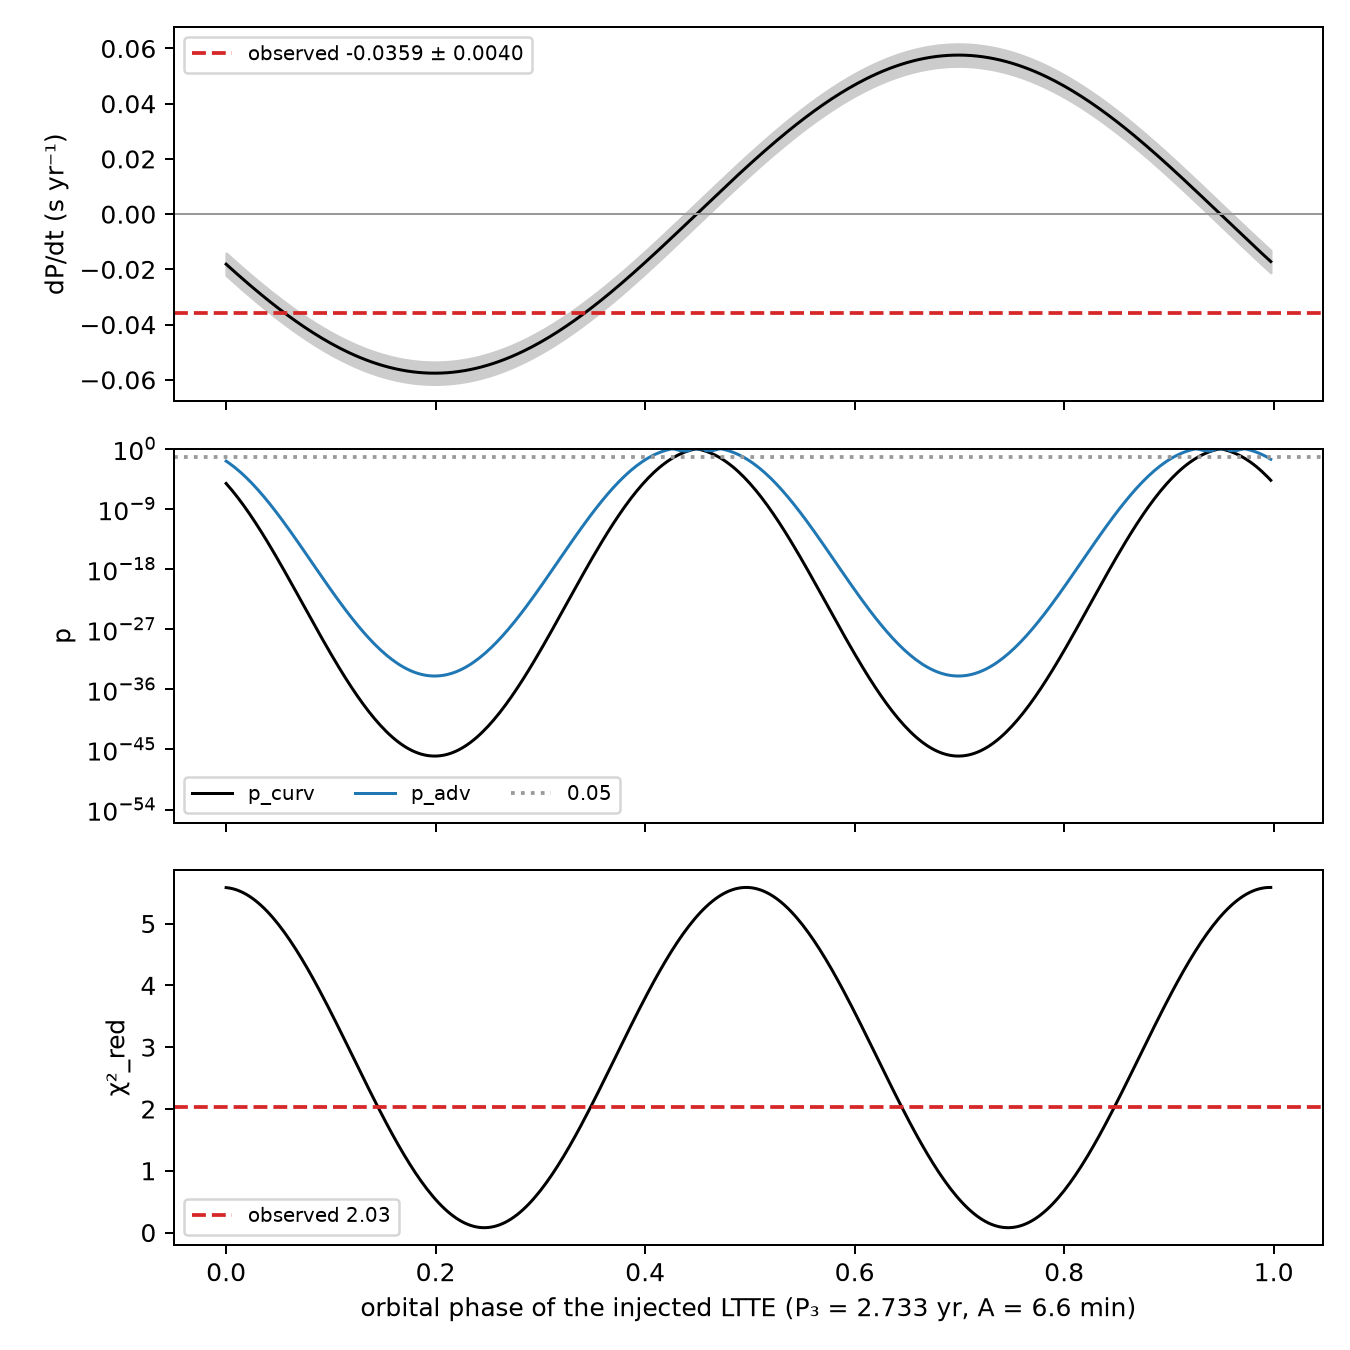
\includegraphics[width=\linewidth]{figures/fig2_v527_injecao.png}
\caption{The published LTTE orbit of V527 Dra injected on a linear ephemeris at our six epochs, over 360 orbital phases: the resulting quadratic coefficient (top), the curvature and adversarial p-values (middle) and the reduced $\chi^2$ (bottom) against phase, with the values our chain returns for the target marked ($\mathrm{d}P/\mathrm{d}t$ = $-$0.0368 $\pm$ 0.0033 s\,yr$^{-1}$, $p_{\rm gof}$ = 0.11).}
\label{f:v527}
\end{figure}

\subsection{The window test: the same coefficient from the complete TESS block, and the external records}\label{ss:externo}
The three mechanisms above are internal. This section confronts each design with two things it did not use: the complete TESS block of the same target, and the published record where one exists.

\textbf{The test.} For the nine members of D9 the coefficient was refitted to every primary epoch the cache holds --- 38 to 43 sectors over 2019.6--2024.9 for eight of them, against the four the design uses --- under each of the noise models of Sect.~\ref{sss:teto}, and compared with the tabulated coefficient as z = ($\mathrm{d}P/\mathrm{d}t$\_TESS $-$ $\mathrm{d}P/\mathrm{d}t$\_design)/the quadrature sum of the two bars. One target, V Gru (TIC 144194304), has only four cached sectors and is not testable. Classes follow a rule fixed before the comparison was read: \textit{contradicted} if |z| > 3 under every admitted model, \textit{not contradicted} if |z| < 2 under every admitted model, \textit{ambiguous} otherwise, where admitted has the meaning of Sect.~\ref{sss:teto}. V527 Dra is held out of this classification, because its published light-travel-time orbit is precisely a signal the TESS block would have to fit, and it is reported instead by the complete fit (Sect.~\ref{ss:orb}). The classification does not depend on the shared epochs: repeating it with the four design epochs removed from the block --- leaving 35 to 39 epochs that share nothing with the tabulated fit --- changes no class, moves no z by more than 0.09 and no bar by more than 1\%.

\textbf{The result is that the block contradicts four of the seven coefficients it classifies and agrees with power in one.} Seven of the eight testable targets are classified (V527 Dra is held out), and \textbf{four of the seven are contradicted} (the threshold |z| > 3 was fixed with the class criterion, before the comparison was read; at |z| > 4 the count is 1, TIC 392536812). Every block coefficient below is the one of the least favourable admitted model, the same the table carries, so that the number and the class in a line come from one model:

\begin{itemize}
\item \textbf{TIC 392536812} --- block +0.0209 $\pm$ 0.0074 under its three admitted models against a tabulated +0.0536 $\pm$ 0.0029: z = $-$4.1. (The pooled-GP variant listed in Table~\ref{t:janela} has a bar three times larger and does not reach 2$\sigma$; it is not an admitted model for this target.)
\item \textbf{TIC 198408416} --- +0.0468 $\pm$ 0.0107 against +0.0099 $\pm$ 0.0011: z from +3.4 to +6.1.
\item \textbf{TIC 390021728} --- +0.0286 $\pm$ 0.0088 against -0.0052 $\pm$ 0.0010: z from +3.8 to +5.5, and the block gives the \textit{opposite sign}.
\item \textbf{TIC 232634196} --- -0.6485 $\pm$ 0.1328 against -0.2181 $\pm$ 0.0207: z from $-$9.5 to $-$3.2.
\end{itemize}

Two are not contradicted --- TIC 230386284 (+0.0091 $\pm$ 0.0008 against +0.0081 $\pm$ 0.0006, z = +1.0) and TIC 377253090 (-0.0050 $\pm$ 0.0049 against -0.0061 $\pm$ 0.0010, z from $-$0.0 to +0.2) --- and one is ambiguous, V564 Dra (TIC 329246824), whose only admitted model gives z = +2.9. V527 Dra, held out, is compatible with zero against its tabulated $-$0.0368 $\pm$ 0.0033 on both readings: -0.0090 $\pm$ 0.0564 from the block under its single admitted model (Table~\ref{t:janela}), and -0.0065 $\pm$ 0.0071 to +0.0012 $\pm$ 0.0264 over the four models fitted to the whole record. Widening or narrowing the admission interval to 99\% or 90\% changes no class.

\textbf{What ``not contradicted'' is worth.} The minimum difference the block could have detected at 3$\sigma$ under the admitted model is 0.0024 s\,yr$^{-1}$ for TIC 230386284 and 0.0146 for TIC 377253090. The first is a third of the tabulated coefficient: the complete block agrees with the design there \textbf{at a power that would have shown a disagreement of a third of the value}, which is the strongest agreement in the sample. The bars of TIC 230386284 look conservative on two independent scales --- its design fit has $\chi^2_{\rm red}$ = 0.07 with $\nu$ = 2, at the 7th percentile of $\chi^2$\_$\nu$/$\nu$, and its extended block gives $\chi^2/\nu$ = 0.17--0.28 --- so the agreement was tested against design bars deflated by 2 and by 3: z rises from +1.02 to +1.18 and +1.21, towards the threshold but still far below it. The reason it moves so little is that the denominator is dominated by the \textit{block's} bar (0.00081 against 0.00057 s\,yr$^{-1}$ for the design): deflating the design bar by three shrinks the quadrature sum by only 16\%, and the difference itself does not move at all, since neither coefficient depends on the design bars' scale. The second is 2.4 times the coefficient, so that target is untested rather than confirmed --- and the three facts about it belong in one place: its design detection does not survive a common archival offset of 2 min (Table~\ref{t:coef}), the block could only have shown a difference of 0.0146 s\,yr$^{-1}$ against a coefficient of 0.0061, and it is the target with an unresolved companion of nearly equal brightness at 1.7\arcsec (Sect.~\ref{ss:epocas}). The two members of ``not contradicted'' are not equivalent: one is the strongest agreement in the sample and the other is the weakest test in it. For the ambiguous and the contradicted targets the same quantity runs from 0.020 to 0.40 s\,yr$^{-1}$. One reading of the four contradictions is excluded by their own pattern: if they were selection effects --- the largest coefficients of a noisy sample regressing to the mean when re-measured --- the block would return systematically \textit{smaller} values. It does not: three of the four are larger in the block than in the design and one has the opposite sign, which is not what regression to the mean produces. \textbf{No target is confirmed as a secular rate by this test}: agreement within the achievable power is the strongest statement any of them supports.

\textbf{What the block shows, and what it does not separate.} Grouped by calendar year against the quadratic fitted to everything, three of the four contradicted targets show a wander of 2.4 to 8.5 min (TIC 198408416 2.4, 390021728 2.6, 232634196 8.5) against within-year dispersions of 0.2 to 2.2 min and bars of 0.1 to 0.8 min; the excursions peak in 2021--2022 and return, and in TIC 232634196 a cubic term is required ($\Delta\chi^2$ = 39 for one parameter, p $\approx$ 4 $\times$ $10^{-10}$). \textbf{The fourth contradicted target is contradicted by the value of its coefficient and not by a wander}: TIC 392536812 moves by 0.82 min over the six years, against 0.11 and 0.66 min in the two uncontradicted targets and 1.49 min in the ambiguous one, so the size of the excursion does not separate the classes --- a target can disagree with its own tabulated coefficient while its block is quiet. V527 Dra, held out, shows 8.2 min. Nor is the wander a higher-order polynomial: outside TIC 232634196 a cubic term adds $\Delta\chi^2$ $\le$ 3.5 for one parameter in every target, so what the block sees is structure on a scale of years that no polynomial of the degrees tested describes. This is the same statement as Sect.~\ref{sss:teto} seen in the time domain: what the design reads as curvature over 16--20 yr is, in the targets where the block can see it, a wander of minutes over years. Wander of that size in close binaries is not new --- Tran et al. (2013) report it, with larger amplitude and in a sample an order of magnitude larger, from Kepler --- and the external corroboration matters here more than the novelty: the behaviour this paper finds in eight targets is the behaviour a bigger survey already found in hundreds. What Sect.~\ref{sss:secundarios} adds is that in six of these eight it does \textit{not} carry the anticorrelation that the same literature attributes to spots.

\textbf{Why the contradictions do not depend on the archival error budget.} z is a difference divided by the quadrature sum of two bars, and in each of the seven the bar of the complete block dominates that sum: a systematic on the design side --- the chain bias of Sect.~\ref{ss:vies}, the per-target shape bias, any common offset of the archival block --- moves the numerator a little and the denominator almost not at all. Imposing the 3 min common offset of Sect.~\ref{sss:teto} on every target leaves all four contradictions above 3$\sigma$ (TIC 198408416 3.5; TIC 232634196 3.2; TIC 390021728 3.7; TIC 392536812 3.8), and a scan from 0.75 to 10 min shows what it would take to end each of them: TIC 198408416, TIC 232634196, TIC 390021728 stay above 3$\sigma$ at every block up to 10 min; TIC 392536812 crosses at 10 min. The objection that the archival error budget is incomplete is correct --- the shape bias was measured before it was propagated, and its season-to-season part is still not --- and the contradictions are not what it reaches.

\textbf{The second axis: how much the design detection itself can take.} The same scan asks a different question of each detection: the smallest common archival offset that removes it, given in the last column of Table~\ref{t:coef}. Over the eleven, the offset that defeats the detection is TIC 377253090 at 2 min; TIC 390021728 at 2 min; TIC 229914020 at 2.5 min; TIC 198408416 at 5 min; TIC 230386284 at 5 min; TIC 144194304 at 7 min; TIC 198388252 at 7 min; TIC 329246824 at 7 min; TIC 424461577 at 10 min; TIC 232634196 and TIC 392536812 beyond 10 min. Crossed with the class of this section, the two axes are independent, and one target sits at the corner of both: \textbf{TIC 390021728 is the cleanest window coefficient in the sample} --- its design detection does not survive a common archival offset of 2 min, and its own complete TESS block contradicts the coefficient at more than 3$\sigma$. What that does not say: it is not evidence that the tabulated value is a mismeasurement. The two axes say that it survives neither test, not that its number was computed wrongly, and --- as Sect.~\ref{s:claim} states for every contradiction --- a disagreement between two windows does not identify what produced it.

\textbf{The external records.} Published work on the 26 was reviewed by position (SIMBAD 5\arcsec: 26 of 26 matched; the VarAstro catalogue 1\arcmin: 13 of 26 have an entry, 6 have $\ge$ 4 CCD primary minima spanning 7.7--34 yr). No target has a published $\mathrm{d}P/\mathrm{d}t$; five have object-scale papers --- V527 Dra (Čeki et al. 2024), HD 202042 (Pawar et al. 2026), and three with photometric studies that do not fit a period change (Pyatnytskyy 2020; Tanrıver et al. 2023) --- of which one, V527 Dra, has a published light-travel-time orbit and no secular term (Sect.~\ref{ss:orb}). Two targets have an external record long enough to test a secular reading, and they say the same thing as the block. \textbf{CV Dra} (TIC 229687624) has 83 CCD minima over 1988--2022: a quadratic over the whole record gives +0.0088 $\pm$ 0.0005 s\,yr$^{-1}$ against our $-$0.0013 $\pm$ 0.0021 (z = $-$4.7), while the same fit restricted to our own window gives $-$0.0003 $\pm$ 0.0017 (z = $-$0.4). Its O$-$C runs from +5 min in 1988 through $-$10 min in 2002 to +8 min in 2022, with quadratic residuals reaching 9.6 min against an intra-year scatter of 2.4 min (Fig.~\ref{f:cvdra}). \textbf{V564 Dra} (TIC 329246824) has 10 CCD minima over 1999--2025: $-$0.0066 $\pm$ 0.0011 s\,yr$^{-1}$ over the whole record against our $-$0.0204 $\pm$ 0.0026 (z = $-$5.0), and $-$0.0130 $\pm$ 0.0042 within our window (z = $-$1.6) --- the same sign, a third of the size, and the disagreement is with the window and not with the measurement. It is also the target the complete TESS block calls ambiguous. At the level of the data rather than of the coefficients, our epochs placed on the VarAstro ephemeris next to CCD minima taken within a year agree in 2 of 2 comparisons in the SuperWASP era (differences $-$1.1 and +2.8 min, rms z = 0.80) and in 12 of 13 in the TESS era (rms z = 1.17); for V391 Dra (TIC 237116051) the cross-match is not usable, because VarAstro adopts half the catalogue period and 5 of its 7 ``primary'' minima are secondary minima under the convention of Table~\ref{t:coef}.

\textbf{TIC 232634196, and the prediction that decides it.} TYC 3906-474-1 (Tmag 9.9, P = 1.2511 d) has the largest tabulated coefficient of the sample, $-$0.218 $\pm$ 0.021 s\,yr$^{-1}$, and it is the one detection carried by the archival lever: on the 20-yr linear ephemeris of the primaries the three SuperWASP seasons sit at $-$137, $-$100 and $-$110 min with 19.9-min bars, and the quadratic through them predicts the change seen inside the TESS block of the design. Its secondary moves in the same direction as its primary ($-$2.4 $\pm$ 0.9 min against $-$11.2 $\pm$ 1.5 min between 2019--2020 and sector 75), which excludes the anti-correlated signature of apsidal motion; the cycle count across the gap is unambiguous ($\sigma_P \times N$ = 0.002); there is no VarAstro record and no literature on the star.

The complete block does not sustain the secular reading. Fitted to the 43 cached sectors alone, the coefficient is $-$0.65 $\pm$ 0.13 s\,yr$^{-1}$ under the admitted model ($-$0.70 $\pm$ 0.05 under the pooled one), three to nine sigma from the tabulated value; fitted to everything, $-$0.29 $\pm$ 0.02 with a reduced $\chi^2$ of 4.1; and the year-by-year O$-$C of the block against that fit runs $-$2.1, +4.9, +2.9 and $-$1.9 min in 2020, 2021.5, 2022--23 and 2024, an excursion of 8.5 min that a cubic term improves by $\Delta\chi^2$ = 39 for one parameter. The local period of 2024, from the eleven sectors 76--86, is +0.46 $\pm$ 0.44 s away from the mean period of the ladder, where the quadratic fitted to everything requires $-$0.75 $\pm$ 0.06 s: a 2.7$\sigma$ conflict, and the local ephemeris agrees with the \textit{linear} one instead.

Instead of developing the object further the paper publishes the prediction that separates the ephemerides. The star (RA 17h58m, Dec +56$^\circ$) is near solar conjunction in January and observable from May to August, so the prediction is given for the observing season: for cycle E = 2206, the primary minimum nearest 2027.5, the quadratic fitted to everything gives BJD\_TDB 2461588.806 $\pm$ 1.8 min, the linear one 2461588.821 (+20.8 min later) and the 2024 local ephemeris 2461588.822 (+21.7 min, $\pm$ 6.5). Scaled by the square root of the reduced $\chi^2$ of each fit --- necessary, since the fits do not describe the data --- the windows become $\pm$3.7, $\pm$3.9 and $\pm$9.5 min and the separation between the linear and the quadratic prediction is 3.9$\sigma$. A single minimum timed to a minute in mid-2027 therefore decides between them, and the 2024 local ephemeris already sits on the linear side. \textbf{This is a test between two ephemerides, not a confirmation of either.}

\textbf{A prediction registered in advance.} When TESS returns to the northern field, the sectors after s86 will give the same test out of sample. The prediction is registered here by class and precedes any sector later than s86, because no such sector exists: the MAST inventory of Sect.~\ref{s:sel} returns nothing after s86 for the eight, TESS having observed the south in 2025--2026. The script that will run the test when those sectors arrive, \texttt{ffi\_\allowbreak fora\_\allowbreak amostra\_\allowbreak d9}, carries the prediction in its docstring in the public code repository, and the deposit archived at Zenodo (Data availability) carries the date stamp. For the targets \textit{not contradicted} the quadratic fitted to everything should win over the 2024 local linear ephemeris, with $\chi^2$/n below 2; for those \textit{contradicted} the 2024 local ephemeris should win, and the 7-epoch quadratic should lose by the largest margin; for the target classed as ambiguous no prediction is made. A not-contradicted target in which the local ephemeris wins, or a contradicted one in which the design quadratic wins, refutes the reading of this section.


\section{What is and is not claimed}\label{s:claim}
Claimed:

What the estimator does, before any target is discussed. These five are properties of the chain, measured on the same 26 designs and independent of which coefficient is real.

\begin{itemize}
\item the coefficients of Table~\ref{t:coef} and their distribution in the partitions of Table~\ref{t:dist} --- sign-symmetric, with a median $|\mathrm{d}P/\mathrm{d}t|$ that depends on the partition --- for the subpopulation defined by Tables~\ref{t:funil}--\ref{t:naomedidos}, \textbf{as quadratic coefficients over 16--20 yr and not as rates};
\item that with formal timing errors the same chain would have reported 20 of these same 26 targets as significant period changes and 19 as surviving the adversarial gate, against 11 with the bars of Sect.~\ref{ss:barras} (24 of 31 over the wider set that reaches a fit with formal errors);
\item that with bars co-estimated from two or three samples the residual test has a null of 0.77, not 1; that the apparent archival excess of 2.73 was a misplaced $\sqrt{n}$ measured against that wrong null, and the remainder, 1.31, is located in three targets whose quadratic the goodness-of-fit test rejects; and that over the 23 targets with an adequate quadratic neither archive shows excess against the null with the same cut applied inside it (SuperWASP 0.72, TESS 0.68), so no bar correction is applied --- with the limit that the test does not separate correct bars from bars inflated by a real secular term of the tabulated size;
\item that the completeness of the chain for a secular term, with the same estimator, is 50\% at 0.014 s\,yr$^{-1}$, and that the co-estimated bars suppress the significance of a real term by a factor that grows with it (median 2.9 at 0.2 s\,yr$^{-1}$, up to 24 in the targets with the smallest archival bars), leaving the coefficient unbiased and the goodness-of-fit test blind;
\item that the epochs do not depend on the timing template: refitting the archival epochs with the profile width free instead of taken from the catalogue moves the coefficients by a median of 0.11$\sigma$ and leaves all eleven detections standing, so the $\pm$3 min shape bias of Sect.~\ref{ss:vies} is a bias of phase coverage and profile mismatch and not of width;
\end{itemize}

What the archival lever is worth. The 16--20 yr baseline is what makes a coefficient measurable at all, and it is carried by two or three epochs whose offset is calibrated on four objects.

\begin{itemize}
\item that the archival timing bias is $-$1.26 $\pm$ 0.75 min when calibrated against ephemerides that include ground-based timings; that it is not reproduced by the estimator acting on the transit shape ($-$0.10 min), does not come from the time-system conversion (0.002 s), and rests on one of the four calibrators; and that its uncertainty is a first-order term in the tabulated coefficients (more than 1$\sigma$ in 16 of 26 between 0 and $-$4.28 min) and a zeroth-order term in the verdicts;
\item that the smallest common archival offset which removes each detection, from a scan of 0.75 to 10 min, is given in Table~\ref{t:coef}, and that it separates the detections into those that survive an offset larger than the bias itself and those that do not;
\item that a second cut, on the archival side rather than the TESS one, leaves \textbf{8 of the 11} when a common offset of 3 min is imposed on each target's archival block (TIC 144194304, 198388252, 198408416, 230386284, 232634196, 329246824, 392536812 and 424461577), that it is not the same 7 the noise model leaves, and that \textbf{6 survive both} (TIC 144194304, 198408416, 230386284, 232634196, 329246824 and 392536812);
\end{itemize}

What the TESS lever is worth. The block of 38 to 43 sectors is the part of the record with no archival bias in it, and it has a noise floor of its own.

\begin{itemize}
\item that the between-sector timing noise is measured, not assumed: a white excess of 0.42 min (median, against a quadratic) required at 95\% in 17 of 21 informative targets, correlated with $\tau$\_c $\approx$ 68 d and an amplitude of 0.8 min pooled, and not a random walk at 2$\sigma$; that under a noise model admitted by its own goodness of fit on the extended block, \textbf{7 of the 11 detections survive} (TIC 144194304, 198408416, 230386284, 232634196, 329246824, 377253090 and 392536812), of which three are contradicted by the complete block of Sect.~\ref{ss:externo}; and that the pooled amplitude, which is what makes the error bar of the window test, is not calibrated in any of the eight targets where the complete block can test it ($\chi^2/\nu$ from 0.05 to 6.4);
\item that the mean and the difference of the primary and secondary minima, over the same complete blocks, \textbf{bound} the anticorrelated component that spots produce: the test detects it in one of the eight targets it carries, finds the two minima moving together in 6, and puts a 95\% upper limit on it that, against the year-to-year wander a smooth term does not explain, falls below that wander in 2 of the eight and below half of it in none --- so the bound is real and, in six of the eight, too loose to exclude an anticorrelated pattern as the cause of anything; and that in the one target where both an orbit and documented spots exist (V527 Dra) the bound is 0.49 min peak-to-peak against a 7.3 min wander --- documented spots need not produce an anticorrelated timing signature of this size, so a non-detection here is not a statement about spots;
\end{itemize}

What happens when the two levers are confronted, and when either is confronted with an external record.

\begin{itemize}
\item that the complete TESS block, 38 to 43 primary epochs per target and 35 to 39 of them independent of the design when the shared epochs are removed, \textbf{contradicts four of the seven coefficients it classifies at more than 3$\sigma$ under every admitted noise model} (TIC 198408416, 232634196, 390021728 and 392536812 --- one of them with the opposite sign) and leaves one ambiguous; that of the two it does not contradict, TIC 230386284 agrees at a power of 0.0024 s\,yr$^{-1}$, a third of its coefficient, and TIC 377253090 is untested at its own power of 0.0146 s\,yr$^{-1}$; and that none is confirmed as a secular rate;
\item that V527 Dra, whose published O$-$C is a light-travel-time orbit with no secular term, passes the significance, adversarial and goodness-of-fit tests on the design and is corrected by the complete block, whose coefficient is compatible with zero;
\item that where an independent 34-yr record exists (CV Dra), the same window reproduces the coefficient and the whole record does not.
\item that undersampled orbits of the declared population, injected on the same correlated noise and judged by the same tests, account for N = 1.25 detections (95\% Jeffreys 0.80--2.46), with a false-alarm rate of zero in that metric;
\end{itemize}

Not claimed:

About the coefficients.

\begin{itemize}
\item \textbf{that any tabulated coefficient is a secular rate.} None is confirmed: of the seven the complete block classifies, four are contradicted and one is ambiguous, one agrees at a power of 0.0024 s\,yr$^{-1}$ and one is untested at 0.0146; V527 Dra is a published orbit and V Gru is not testable with four cached sectors;
\item that the tabulated $\sigma(\mathrm{d}P/\mathrm{d}t)$ is the measurement error of a real secular term: for a term of 0.1--0.2 s\,yr$^{-1}$ on designs with 1.5--5 min archival bars it is an overestimate by up to an order of magnitude;
\item that a target not contradicted by the complete block is confirmed by it;
\item that the timing of TIC 377253090 is free of its unresolved 1.7\arcsec companion of equal brightness: a constant companion does not move a minimum, but its variability was not tested;
\item the functional form of any O$-$C diagram; the presence of third bodies in any system beyond the published one; the physical mechanism behind any individual coefficient;
\end{itemize}

About the tests.

\begin{itemize}
\item that the adversarial test has a significance level: it is a robustness gate (Sect.~\ref{ss:testes});
\item that the noise model of Sect.~\ref{sss:teto} is unique. It is the one admitted by its own goodness of fit on the extended block, chosen by a criterion written after the models were compared and using $\chi^2/\nu$ alone; the pooled alternative gives the same count with a different membership, and the choice changes which targets survive, not how many;
\item that the TESS bars inflated by 1.0 min\,yr$^{-1}$ are calibrated (they are a ceiling);
\item that the mean of the two minima removes spot timing noise in general: it cancels only the anticorrelated component, and polar or persistently placed spots survive it;
\item that the contradictions identify the \textit{origin} of what the block sees --- the wander of minutes over years is not attributed here to spots, to a third body or to period change --- nor that every contradiction comes from such a wander: one of the four (TIC 392536812) is contradicted by the value of its coefficient while its own block is quiet (Sect.~\ref{ss:externo}).
\item any bound on the in-window tertiary fraction from the residuals of this sample: the TESS side excludes nothing below the highest published fraction (Sect.~\ref{sss:orbitas});
\end{itemize}

About the transfer of the bias, and of the corrections.

\begin{itemize}
\item that the chain bias transfers from hot Jupiters to deep, short eclipses --- it is carried as a declared limitation, bounded only by two archival minima of CV Dra (n = 2). What is no longer claimed as a limitation is the earlier one, that the bias rests on a single calibrator: it is measured on all 6 objects the archive allows, and dropping the most precise of them leaves -1.08 $\pm$ 0.97 min rather than the $-$0.46 $\pm$ 1.04 that the four gave;
\item that the part of the per-target shape bias which varies from season to season is propagated: only its common part is corrected, the rest enters the archival dispersion and, by the coupling of Sect.~\ref{sss:secular}, suppresses significance rather than creating it;
\end{itemize}

The flagged targets are not developed as case studies here. Earlier readings withdrawn in the course of the work are listed in Appendix~\ref{a:C}.


\section{Data and code}\label{s:data}
\begin{sloppypar}
Catalogues: Prša et al. (2022; VizieR J/ApJS/258/16), Kostov et al. (2025; J/ApJS/279/50). Photometry: TESS (Ricker et al. 2015) SPOC 2-min light curves (Jenkins et al. 2016) from MAST; SuperWASP public archive (Butters et al. 2010) as served by CERIT-SC (\url{https://wasp.cerit-sc.cz}). Published timings: VarAstro star catalogue and O$-$C data (var.astro.cz; Paschke \& Brát 2006), queried 2026-09-13; bibliographies from SIMBAD (Wenger et al. 2000) and catalogues from VizieR (Ochsenbein et al. 2000), both queried 2026-09-13. Published ephemerides for the timing-bias calibration: Ivshina \& Winn (2022; VizieR J/ApJS/259/62), Kokori et al. (2023; J/ApJS/265/4) and Bouma et al. (2020). Software: astropy (Astropy Collaboration 2013, 2018, 2022), numpy, scipy, pandas.

\end{sloppypar}

\section{Data availability}\label{s:avail}
\begin{sloppypar}
The code that produces every number in this paper is developed in a public repository (\url{https://github.com/rondinellewalitte/dpdt-26-binaries}) and archived at Zenodo under the concept DOI \url{https://doi.org/10.5281/zenodo.22740628,} which always resolves to the latest version. The version DOI 10.5281/zenodo.22740629 archives the code as it stood before the revisions recorded in the appendix of changes of state and in the deposited record of defects of the publication chain; the version that matches this manuscript is deposited under the same concept DOI at submission, and a further version DOI will be minted at acceptance. Three files of the archive were appendices of earlier versions of this manuscript and were moved to the deposit when it was cut for length, unchanged: \texttt{reports/apendice\_\allowbreak a\_\allowbreak recuperacao.md} (the outcome of the recovery pass, per target, summarised in Table~\ref{t:naomedidos}), \texttt{reports/apendice\_\allowbreak d\_\allowbreak retiradas.md} (the sixteen readings withdrawn between versions, with what replaced each) and \texttt{reports/apendice\_\allowbreak d\_\allowbreak defeitos\_\allowbreak publicacao.md} (the five defects of the publication chain and the guard each one produced). The archive holds, besides the chain itself (\texttt{cadeia\_\allowbreak oc}, \texttt{oc\_\allowbreak lote}, \texttt{superwasp}, \texttt{epocas\_\allowbreak 142874476}, \texttt{ids}) and the table, figure and manuscript generators (\texttt{tabela\_\allowbreak nota}, \texttt{figuras\_\allowbreak nota}, \texttt{epocas\_\allowbreak cds\_\allowbreak 26}, \texttt{md\_\allowbreak para\_\allowbreak tex}, \texttt{numeros\_\allowbreak da\_\allowbreak nota}, \texttt{confere\_\allowbreak nota}), one script per measurement reported here, each with its expectation written in the docstring and committed before the run:

\begin{itemize}
\item \textit{Sect.~\ref{s:sel} and the sample:} \texttt{vies\_\allowbreak cache\_\allowbreak 288} (sector census), \texttt{arquivo\_\allowbreak completo\_\allowbreak 26} (MAST manifest of the 799 light curves), \texttt{ffi\_\allowbreak fora\_\allowbreak amostra\_\allowbreak d9} (product inventory after s86 and the FFI-versus-2-min control).
\item \textit{Sect.~\ref{s:met} and the bias:} \texttt{run\_\allowbreak hj\_\allowbreak calib}, \texttt{vies\_\allowbreak hj\_\allowbreak indep} (calibration against published ground-based ephemerides), \texttt{vies\_\allowbreak forma\_\allowbreak swasp} (shape test), \texttt{checa\_\allowbreak tempo\_\allowbreak swasp} (time-system check), \texttt{sensib\_\allowbreak vies\_\allowbreak 26} (sensitivity of every coefficient and verdict to the bias), \texttt{estimador\_\allowbreak alt\_\allowbreak d11} and \texttt{estimador\_\allowbreak alt\_\allowbreak refit} (the second timing template, with the profile width free, and the refit of the eleven detections with its epochs), \texttt{barra\_\allowbreak tess\_\allowbreak metades\_\allowbreak 26}, \texttt{gls\_\allowbreak vies\_\allowbreak 26}, \texttt{blending\_\allowbreak 26}.
\item \textit{Sect.~\ref{ss:formais}--5.2:} \texttt{qual\_\allowbreak barra\_\allowbreak 26}, \texttt{nulo\_\allowbreak barras\_\allowbreak reestimadas\_\allowbreak 26}, \texttt{nulo\_\allowbreak pisos\_\allowbreak 26}, \texttt{vies\_\allowbreak alavanca\_\allowbreak 26}, \texttt{estrutura\_\allowbreak swasp\_\allowbreak 26}, \texttt{completude\_\allowbreak secular\_\allowbreak 26}.
\item \textit{Sect.~\ref{ss:setores}:} \texttt{secundarios\_\allowbreak 26}, \texttt{jitter\_\allowbreak 232634196}, \texttt{jitter\_\allowbreak primarios\_\allowbreak 26} (799 sectors, $\sigma$\_j and variogram), \texttt{deriva\_\allowbreak gp\_\allowbreak 26} (pooled and per-target Gaussian process), \texttt{reinflar\_\allowbreak tess\_\allowbreak 26} (ceiling), \texttt{ruido\_\allowbreak admitido\_\allowbreak 26} (admitted noise model and the class criterion), \texttt{reconcilia\_\allowbreak hi\_\allowbreak d9} (the four noise models side by side).
\item \textit{Sect.~\ref{ss:orb}:} \texttt{epsilon\_\allowbreak 26}, \texttt{epsilon\_\allowbreak longo\_\allowbreak 26} (long-period bands, strict tertiary count, injection on correlated noise), \texttt{v527\_\allowbreak ltte}.
\item \textit{Sect.~\ref{ss:externo}:} \texttt{caso\_\allowbreak 232634196}, \texttt{caso\_\allowbreak 232634196\_\allowbreak completo}, \texttt{caso\_\allowbreak completo\_\allowbreak d9} (the window test, with and without the design epochs), \texttt{previsao\_\allowbreak 232634196}, \texttt{literatura\_\allowbreak 26}, \texttt{comparar\_\allowbreak brno\_\allowbreak 26}.
\item \textit{State comparisons:} \texttt{comparar\_\allowbreak estados\_\allowbreak BD} and \texttt{comparar\_\allowbreak estados\_\allowbreak DE}, which reproduce what each change of the chain moved (Appendix~\ref{a:C}).
\item Kept for the record of withdrawn corrections: \texttt{reinflar\_\allowbreak swasp\_\allowbreak 26}, \texttt{reinflar\_\allowbreak conjunto\_\allowbreak 26}.
\end{itemize}

The per-target records (\texttt{data/orquestra/oc\_\allowbreak lote/oc\_\allowbreak \_\allowbreak <TIC>.json}) carry every epoch, bar and fit; the derived tables used here are \texttt{tabela\_\allowbreak 26}, \texttt{caso\_\allowbreak completo\_\allowbreak d9}, \texttt{caso\_\allowbreak completo\_\allowbreak d9\_\allowbreak sem\_\allowbreak desenho}, \texttt{ruido\_\allowbreak admitido\_\allowbreak d9}, \texttt{ruido\_\allowbreak admitido\_\allowbreak 26}, \texttt{reconcilia\_\allowbreak hi\_\allowbreak d9}, \texttt{sensib\_\allowbreak vies\_\allowbreak 26}, \texttt{jitter\_\allowbreak primarios\_\allowbreak 26}, \texttt{deriva\_\allowbreak gp\_\allowbreak 26\_\allowbreak hiper}, \texttt{deriva\_\allowbreak gp\_\allowbreak 26\_\allowbreak desenho}, \texttt{epsilon\_\allowbreak longo\_\allowbreak 26}, \texttt{epsilon\_\allowbreak gp\_\allowbreak 26}, \texttt{qual\_\allowbreak barra\_\allowbreak 26}, \texttt{nulo\_\allowbreak barras\_\allowbreak reestimadas\_\allowbreak 26}, \texttt{nulo\_\allowbreak condicionado\_\allowbreak 26}, \texttt{nulo\_\allowbreak pisos\_\allowbreak 26}, \texttt{completude\_\allowbreak secular\_\allowbreak 26}, \texttt{secundarios\_\allowbreak 26}, \texttt{comparacao\_\allowbreak brno\_\allowbreak 26}, \texttt{sobreposicao\_\allowbreak brno\_\allowbreak 26}, \texttt{literatura\_\allowbreak 26}, \texttt{vies\_\allowbreak forma\_\allowbreak swasp}, \texttt{vies\_\allowbreak hj\_\allowbreak indep}, \texttt{ffi\_\allowbreak fora\_\allowbreak amostra\_\allowbreak d9} and the state comparisons \texttt{comparacao\_\allowbreak estado\_\allowbreak B\_\allowbreak D} and \texttt{comparacao\_\allowbreak estado\_\allowbreak D\_\allowbreak E}. The eclipse timings of the 26 targets are also given as a machine-readable table (\texttt{reports/epocas\_\allowbreak 26.csv}, 145 epochs) for CDS. \texttt{numeros\_\allowbreak da\_\allowbreak nota} writes every number quoted in this paper with the file it comes from, and \texttt{confere\_\allowbreak nota} compares the two and fails if any disagrees.

\end{sloppypar}

\appendix

\section{Control target and period-ladder audit}\label{a:A}
Before any new target was measured, the chain was run as a single function on TIC 142874476 and compared, component by component, with its previously recorded result (38 components: epochs, errors, residuals, $\chi^2$, Q, the SuperWASP source, cycle count, seasons, coverage status and the final residuals). Thirty reproduced to the quoted precision; the eight that did not were all downstream of one number --- a quadratic extrapolation to 2007 of +38.9 min that existed only in a comment and that no fitting convention reproduces. The record was corrected to what the code produces. The adversarial test on the control gives p = 0.28 for the TESS-internal curvature (0.003 before the shift): with four epochs and one degree of freedom that detection is fragile, which is why the robust statement about the control is its 10$\sigma$ departure from a constant period, not the curvature. The control was re-run before and after every change reported in this version and reproduced each time; under the chain bias of this version its archival epoch sits 21.8 min from the linear ephemeris (9.8$\sigma$) and 6.4 min from the quadratic (2.9$\sigma$).

\textbf{Period ladder.} The ladder returns epochs and residuals in the caller's order. This was a latent defect: an earlier version returned them in internal time order, and unsorted input produced cycle numbers assigned to the wrong sectors --- caught only because the resulting $\mathrm{d}P/\mathrm{d}t$ of $-$24\,122 s\,yr$^{-1}$ is physically impossible; a milder scramble would have looked like mass transfer. The $|\mathrm{d}P/\mathrm{d}t|$ > 10 s\,yr$^{-1}$ guard of Sect.~\ref{ss:escada} exists because of it. The tolerance rule of Sect.~\ref{ss:escada} (the larger of 3 min and 3$\times$ the median epoch uncertainty) was introduced after the main batch, which ran with a fixed 3 min; re-running all 26 targets under the rule reproduces every tabulated value (1\,024 fields compared across the 26 per-target records; only the wall-clock time differs).


\section{The orbit population, the efficiency, and the occurrence numbers}\label{a:B}
\textbf{Population.} Circular tertiary orbits with $P_3$ log-uniform in 0.1--20 yr (between a sector and the baseline), binary mass uniform in 1.5--2.5 $M_\odot$, tertiary mass uniform in 0.1--1.0 $M_\odot$, isotropic inclination (cos i uniform), phase uniform; the light-travel-time semi-amplitude follows from Kepler's third law, A = $a_3$ $M_3$/($M_{\rm bin}$ + $M_3$) sin i / c, and reproduces the published 6.6 min of V527 Dra for a 1 $M_\odot$ tertiary at 70$^\circ$ and $P_3$ = 2.733 yr with $M_{\rm bin}$ = 2.5 $M_\odot$, the upper edge of the prior (2.0 $M_\odot$ would give 7.3 min); the binary mass used in that check is therefore the prior's edge, not a measured value. The median amplitude of the population is 2.0 min, comparable to the epoch bars. $\varepsilon_3$ (detection and $p_{\rm gof}$ $\ge$ 0.05) sums to 4.2.

\textbf{What sets $\varepsilon$.} The expectation that $\varepsilon$ would track the sampling pattern was not met: the Spearman correlation of $\varepsilon$ with the number of epoch groups is $-$0.07 (p = 0.72) and with N is +0.19 (p = 0.36), while with the median bar it is $-$0.66 --- the bars set the efficiency, not the pattern. Two targets have $\varepsilon$ = 0 (their archival bars make the curvature test powerless at these amplitudes). For orbits as favourable as V527 Dra's, $\varepsilon$ approaches 0.83; that one empirical anchor is biased, since the orbit was published because it is large enough to solve from 1\,832 timings.

\textbf{Occurrence numbers and what each measures.} Occurrence over all outer periods: 96\% of solar-type spectroscopic binaries with P < 3 d after correction for incompleteness, 79\% raw (Tokovinin et al. 2006); a lower limit of 42 $\pm$ 5\% for contact binaries (Pribulla \& Rucinski 2006). Detected fractions in eclipse-timing surveys: 8.5\% of $\sim$2\,600 Kepler binaries with outer periods below $\sim$2\,000 d (Borkovits et al. 2016); 1.2\% of $\sim$80\,000 OGLE-IV binaries (Hajdu et al. 2019); 10 in $\sim$100 TESS full-frame-image targets (Marcadon \& Prša 2024). The detected fractions are convolved with each survey's baseline, cadence and precision; multiplying them by $\varepsilon$ applies an efficiency twice. The in-window fraction of Sect.~\ref{ss:orb} comes from the 33 tertiaries listed for the 42 P < 3 d systems of Tokovinin et al.'s Table~\ref{t:janela}, counted strictly --- the tertiary of the inner pair itself, which gives 8 of 42 in 0.1--20 yr; the two systems that the loose count adds (HIP 16846 and 61910) have their in-window companion in another subsystem. All eight are spectroscopic or visual-orbit detections rather than resolved wide pairs.


\section{Record of readings withdrawn between versions, and of the changes of state}\label{a:C}
\textbf{Changes of state of the chain, in order.} (A) The first batch used the standard error of the season mean as the bar of each SuperWASP season, $\sqrt{2}$--$\sqrt{3}$ too small in 49 of 61 epochs; the residual factor of the archive was 2.73 and the median reduced $\chi^2$ 1.41. (B) Corrected to the season dispersion: the factor fell to 1.35, the median reduced $\chi^2$ to 0.67, one detection was lost (TIC 359552377), and no coefficient moved by more than 0.04$\sigma$. (C) A state that produced no table: the batch was started again with the complete TESS manifest of the 26 in the design --- every cached sector instead of the four the design uses --- and was stopped at 3 of the 88 by the decision to freeze the design before the first public version; the state-(B) records were restored from the repository with no differences and the manifest was moved out of the chain's glob. The question it would have answered is the one Sect.~\ref{ss:externo} answers instead, by refitting the complete block \textit{beside} the design rather than inside it, which keeps the design fixed and makes the comparison a test rather than a redefinition. (D) The TESS bar from the halves of a sector was $|t_a - t_b|/\sqrt{2}$ --- the dispersion of one half given to the whole sector --- and became $|t_a - t_b|/2$: 36 of 84 bars shrank by a median factor of 0.71, one detection was added (TIC 390021728, $p_{\rm adv}$ 0.10 $\rightarrow$ 0.013), the TESS residual factor rose from 1.02 to 1.59, and no coefficient moved by more than 0.20$\sigma$. (E) The archival bias was recalibrated against ephemerides that include ground-based timings and went from $-$2.14 $\pm$ 0.78 to $-$1.26 $\pm$ 0.75 min (Sect.~\ref{ss:vies}): every archival epoch moved by +0.88 min, the 26 coefficients all moved in the same direction by a median of 0.29$\sigma$ (maximum 0.95$\sigma$), the median $|\mathrm{d}P/\mathrm{d}t|$ went from 0.016 to 0.014 s\,yr$^{-1}$, and no verdict, class or flag changed. (F) The per-target shape bias of Sect.~\ref{ss:vies} entered the chain: each target's archival epochs are corrected by the bias measured on its own light curve and template, and the floor of the archival bar became the quadrature sum of the chain bias uncertainty and the uncertainty of that measurement. The corrections are at most 0.80 min among the detections and 2.93 min in the sample (TIC 329248002); three targets whose shape test does not converge (TIC 139256217, 229476285 and 359552377) are left uncorrected with a 3 min floor. The coefficients moved by a median of 0.05$\sigma$ and at most 1.11$\sigma$ (TIC 126945917, a detection in neither state). No detection verdict and no flag changed, and no class of Sect.~\ref{ss:externo} moved; the class column of Table~\ref{t:coef} changed in two targets (TIC 126945917 from $p_{\rm curv}$ 0.081 to 0.004; TIC 329289186 from $p_{\rm curv}$ 0.050 to 0.039), both of which the adversarial gate still rejects --- the entry of state (E) said no class changed, and for (F) that would be false; the median $|\mathrm{d}P/\mathrm{d}t|$ of the 26 went back from 0.014 to 0.016 s\,yr$^{-1}$, because the median falls in a gap of the ordering and the two central targets are 0.014 and 0.017. The state was predicted arithmetically from the state-(E) records before the chain was changed --- the design fit is a deterministic function of epochs and bars --- and the re-run reproduced it exactly: the epochs agree to the last digit written and the coefficients to 2 $\times$ $10^{-11}$ s\,yr$^{-1}$. Each state was run against an expectation committed before the run, and the control target reproduced in all of them; in (F) it reproduced \textit{because} it has no shape measurement, which is also what makes the control blind to this change --- what checks that the change reached only the targets it should is the arithmetic prediction, not the control.

\textbf{Readings withdrawn.} Eighteen readings of earlier versions were withdrawn as the chain was corrected --- a median reduced $\chi^2$ read as bars too small, an archival excess of 2.73 later traced to a composition error, bar corrections built on it, the coefficients and counts that followed, a fraction whose denominator carried the secular term it was meant to exclude, and five confidence intervals on fractions of a sample that is not a sample. Each is recorded, with what replaced it, in \texttt{reports/apendice\_\allowbreak d\_\allowbreak retiradas.md} of the deposit.

\textbf{Defects of the publication chain.} Nine further entries record failures that were not in the measurements but in the path from them to this document --- a display equation left at the value of the previous state, figure files taken from a hand-made copy, an appendix letter assigned by position, body citations left in the previous state after the tables were regenerated, a citation check that reported no divergence over a text that still carried two stale numerals, a cross-reference corrected inside a generated table and restored by the generator, a set of targets that existed only as a list typed into a patch, and two guards that failed without altering anything published. None of them changes a number of this version, so they are recorded in full, each with the guard it produced, in \texttt{reports/apendice\_\allowbreak d\_\allowbreak defeitos\_\allowbreak publicacao.md} of the deposit rather than here; the guards themselves run before any manuscript is produced (\texttt{src/\allowbreak confere\_\allowbreak nota.py}, \texttt{src/\allowbreak citacoes\_\allowbreak tabelas.py}, \texttt{src/\allowbreak md\_\allowbreak para\_\allowbreak tex.py}). The record keeps them because the paper's claim is about method, and a method that produced a correct number and published a wrong one is part of what it has to show.


\section{The residual test: simulations and their expectations}\label{a:D}
This appendix holds the numbers behind Sect.~\ref{ss:qualbarra}: the grids of the simulations, the conditioning of the null, the mechanism that couples a bar to its own residual, and the expectation written and committed before each run. Nothing here is new --- it is the working of the results quoted in the body.

\textbf{The scan of the common archival offset.} The shape bias of Sect.~\ref{ss:vies} is corrected per target (state (F) of Appendix~\ref{a:C}), but the part of it that varies from season to season is not propagated, so what remains is bounded by brute force: a common offset is imposed on every archival epoch of a target, from 0.75 min --- the uncertainty of the chain bias, already in the bars --- to 10 min, and both the design detection and the window test are recomputed at each step. Table~\ref{t:varredura} gives |z| of the window test at each offset (--- for targets outside the test), an asterisk where the design detection no longer survives at that offset, and the smallest offset of the grid that defeats the detection. Two readings come out of it, and they point in opposite directions. The detections go first: at the conservative 3 min, 8 of the 11 survive, and 3 targets lose the detection between 2 to 2.5 min. The contradictions do not go at all: the four are still beyond 3$\sigma$ at 3 min, and two of them barely move across the whole grid, because the bar of the complete block dominates the denominator of z (Sect.~\ref{ss:externo}). The scan is a sensitivity, not a correction: no table in the body is computed with an offset imposed.

\begin{table*}
\caption{The scan of the common archival offset. For the eleven detections (the scan over all 26 targets is in the deposited \texttt{vies\_\allowbreak forma\_\allowbreak propagado\_\allowbreak varredura.parquet}): the class of the window test where the target is in it, |z| of the window test at each imposed common offset of the archival epochs (in min), and the smallest offset of the grid that removes the design detection (``> 10'' when the grid does not reach it). An asterisk marks an offset at which the design detection no longer survives.}
\label{t:varredura}
\centering
\scriptsize
\begin{tabular}{r l r r r r r r r r r r r}
\hline\hline
TIC & class (window test) & 0.75 & 1 & 1.5 & 2 & 2.5 & 3 & 4 & 5 & 7 & 10 & offset that defeats it\\
\hline
144194304 & --- & --- & --- & --- & --- & --- & --- & --- & --- & ---* & ---* & 7\\
198388252 & --- & --- & --- & --- & --- & --- & --- & --- & --- & ---* & ---* & 7\\
198408416 & contradicted & 3.4 & 3.4 & 3.5 & 3.5 & 3.5 & 3.5 & 3.5 & 3.5* & 3.6* & 3.6* & 5\\
229914020 & --- & --- & --- & --- & --- & ---* & ---* & ---* & ---* & ---* & ---* & 2.5\\
230386284 & not contradicted & 1.0 & 0.9 & 0.8 & 0.6 & 0.5 & 0.5 & 0.4 & 0.3* & 0.2* & 0.1* & 5\\
232634196 & contradicted & 3.2 & 3.2 & 3.2 & 3.2 & 3.2 & 3.2 & 3.2 & 3.2 & 3.2 & 3.2 & > 10\\
329246824 & ambiguous & 2.9 & 2.9 & 2.8 & 2.8 & 2.7 & 2.7 & 2.6 & 2.4 & 2.2* & 1.9* & 7\\
377253090 & not contradicted & 0.0 & 0.0 & 0.0 & 0.0* & 0.0* & 0.0* & 0.0* & 0.1* & 0.1* & 0.2* & 2\\
390021728 & contradicted & 3.8 & 3.8 & 3.8 & 3.8* & 3.8* & 3.7* & 3.7* & 3.6* & 3.4* & 3.1* & 2\\
392536812 & contradicted & 4.1 & 4.1 & 4.0 & 4.0 & 3.9 & 3.8 & 3.6 & 3.4 & 3.0 & 2.5 & > 10\\
424461577 & published LTTE & 0.5 & 0.5 & 0.5 & 0.5 & 0.5 & 0.5 & 0.5 & 0.5 & 0.5 & 0.5* & 10\\
\hline
\end{tabular}
\end{table*}

\textbf{Why the null had to be simulated.} For s independent of r, $z^2 = r^2/s^2$ follows $F(1,\nu)$ with mean $\nu/(\nu-2)$, undefined for $\nu \le 2$; an external reader pointed out that with $\nu$ = 1--2 the bootstrap width of the factors was the signature of that, and the expectation written and committed before the simulation was a SuperWASP null of 1.3--1.8, with the then-measured 1.35 inside its central interval. \textbf{The expectation was wrong in direction}: with the bars re-estimated as the pipeline re-estimates them the null is 0.77 (2.5--97.5\%: 0.63--0.94; quartiles 0.72--0.81) and the TESS null 0.98 (median; mean 1.03; 0.54--1.79), both below 1. The reason is not the tied residual of a two-season pair --- the leverage-corrected ratio of such a pair is exactly 1 --- but the floors: removing them in the simulation (\texttt{src/\allowbreak nulo\_\allowbreak pisos\_\allowbreak 26.py}) returns the SuperWASP null to 1.15 and makes the TESS null diverge, because a half-sector dispersion near zero makes z unbounded; the three floors together give 0.78 and 0.95. Treating the 0.75 min bias term as a common offset of the archival block rather than as per-season noise changes nothing (0.76). The values are properties of this design --- 26 targets, 4--7 epochs each, bars co-estimated with $\nu$ = 1--2 and floored by the formal error and the 0.75 min --- and what transfers to another sample is the simulation, not the number.

\textbf{The conditioned null.} The 23 targets with an adequate quadratic are those that passed the goodness-of-fit cut, so the null they are compared with has to apply the same cut inside every realisation: $p_{\rm gof}$ of each target's quadratic computed with the re-estimated bars, the targets below 0.05 removed, the factors formed over the survivors. Under the null the cut removes 0.76 targets per realisation --- 2.9\% per target rather than 5\%, because the re-estimated bars deflate $\chi^2$ --- and three or more in 4.3\% of realisations, so the number of flagged targets in the data is itself a mild excess. The conditioned nulls are 0.77 (0.64--0.92) for SuperWASP, unchanged, and 0.81 (0.46--1.22) for TESS, below the unconditioned 0.98: the realisations that fail the cut are those in which a TESS bar co-estimated from two half-sectors came out small, and they hold 23\% of the TESS $\Sigma z^2$ of the null in 3\% of the target-realisations. Under the TESS bar of the previous version the drop was larger (0.96 to 0.70), against an expectation of 0.85--0.93 written before that run. An earlier version compared the 23 with the null of the same designs \textit{without} the cut (0.78), which is not the same experiment; the external reader pointed this out, and the same conditioning was propagated to the orbit injection below.

\textbf{A secular term through the residual test.} With a term injected in every target and the goodness-of-fit cut applied inside each realisation (\texttt{src/\allowbreak completude\_\allowbreak secular\_\allowbreak 26.py --fator}; expectation written and committed before running: a monotonic fall, about 0.70 at 0.02 s\,yr$^{-1}$), the SuperWASP factor is 0.76, 0.71, 0.59, 0.43 and 0.29 at 0.005, 0.01, 0.02, 0.05 and 0.2 s\,yr$^{-1}$, while the TESS factor stays at 0.81--0.85 --- half-sector bars do not see the term and the parabola absorbs it exactly. With the bars held fixed the factor is 0.99--1.01 at every amplitude: the term lies in the model space and the whole effect is the re-estimation. The measured 0.72 of the 23 sits at the 34th percentile of the null in this run (24th in the run of the conditioned null; Monte Carlo scatter) and at the 58th of the distribution with 0.01 s\,yr$^{-1}$ in every target; P($\le$ 0.72) is 0.88 at 0.02 s\,yr$^{-1}$ and 1.00 at 0.05. The probability of a factor $\ge$ 1.31 is 0.001 with no term and 0.04--0.08 with 0.01--0.05 s\,yr$^{-1}$ in every target: a population of real terms of the tabulated size is not excluded as the source of the excess of the 26, although the three flagged targets remain the simpler account of where it sits.

\textbf{The coupling between bar and residual.} The reading first written for the fall of the factor --- that the inflated archival bars hand the fit to the TESS block --- was tested and is wrong: the mean leverage of the archival epochs stays at 0.41--0.42 across the grid. What the term breaks is the coupling between a bar and its own residual. With two seasons the bar is $|\Delta|/\sqrt{2}$ and the residual $\pm\Delta/2$ of the same between-season difference $\Delta$; with a term, the bar is built from the signal's between-season difference plus the noise's, and the residual --- the parabola having absorbed the term --- from the noise's alone, so that when the two nearly cancel the bar drops to its floor while the residual does not.

\textbf{Orbits through the same estimator.} The injection of the declared population of Sect.~\ref{ss:orb} into the 26 designs, with the bars re-estimated inside the simulation (\texttt{src/\allowbreak estrutura\_\allowbreak swasp\_\allowbreak 26.py}; expectation written and committed before running: the null reproduced at f = 0, a SuperWASP factor of 0.95--1.10 and a TESS factor near 1.5 at f = 0.24), reproduces the null at f = 0 (0.77) and gives, at the occurrence f = 0.24 at which it was run --- the loose count of the earlier version, so an upper bound --- a SuperWASP factor of 0.85 (below the expectation) and a TESS factor of 1.68. The probability that orbits alone produce the measured SuperWASP factor of 1.31 is 0.002 at f = 0, 0.022 at f = 0.24 and 0.16 at f = 1; the TESS factor of 1.59 is as compatible with the declared population at the Tokovinin et al. fraction as with none, which is why the TESS side bounds nothing useful. The first run of this injection held the bars fixed, whose null is 1.00 against the measurement's 0.77; the numbers it gave are withdrawn as cross-estimator comparisons (Appendix~\ref{a:C}).

\textbf{Completeness and self-suppression, in detail.} Over the 23 targets that reach 50\% completeness, the amplitude at which they reach it correlates with the median archival bar (Spearman +0.46, p = 0.03) and, more weakly and in the opposite sense, with the number of epochs ($-$0.26, p = 0.23); with 23 targets, and bar size and epoch count themselves correlated, the two are not separated here, and the three targets that never reach 0.5 are the three with the largest archival bars. Re-estimating the bars costs 12 points of completeness at 0.02 s\,yr$^{-1}$ (median 0.86 against 0.98) and nothing from 0.05 upward. The suppression factor $\sigma(\mathrm{d}P/\mathrm{d}t)$ with re-estimated bars over $\sigma$ with the true bars has a median of 1.03 at 0.02 s\,yr$^{-1}$, 1.19 at 0.05, 1.6 at 0.1 and 2.9 at 0.2, reaching 5--24 at 0.2 in the nine targets whose archival seasons have bars of 1.5--5 min at the longest lever; at the coefficients of Table~\ref{t:coef} the factor for the eleven members of D11 is 0.90--1.71 (median 1.24), and for the TESS side alone 0.90--1.59. The goodness-of-fit cut does not see the term ($p_{\rm gof}$ < 0.05 in 2--4\% of realisations at the median, at most 21\% in one four-epoch design). Two expectations were committed before this run, the external reader's and the author's, and they differed on the size of the suppression; the measured factor exceeded both at the largest amplitudes.

\textbf{The classification the pooled GP would give, and why it is not a sensitivity.} The pooled amplitude (A = 0.835 min, Sect.~\ref{sss:teto}) is the only noise model comparable across targets, and it is the one Table~\ref{t:janela} carries in its own column; classifying with it is a different matter, because it is admitted in none of the eight. Side by side with the $\chi^2/\nu$ that rejects it, target by target: TIC 329246824 z = +0.8 with $\chi^2/\nu$ = 0.30 (not contradicted); TIC 392536812 z = -1.6 with $\chi^2/\nu$ = 0.45 (not contradicted); TIC 198408416 z = +2.9 with $\chi^2/\nu$ = 0.33 (ambiguous); TIC 230386284 z = +0.1 with $\chi^2/\nu$ = 0.05 (not contradicted); TIC 377253090 z = +0.3 with $\chi^2/\nu$ = 0.56 (not contradicted); TIC 390021728 z = +3.1 with $\chi^2/\nu$ = 1.98 (contradicted); TIC 232634196 z = -9.4 with $\chi^2/\nu$ = 2.16 (contradicted); TIC 424461577 z = +3.3 with $\chi^2/\nu$ = 6.37 (held out). Under it 2 of the 7 classified targets would be contradicted, against four under the admitted models. Compared with that classification, three targets change: TIC 329246824 (ambiguous $\rightarrow$ not contradicted), TIC 392536812 (contradicted $\rightarrow$ not contradicted), TIC 198408416 (contradicted $\rightarrow$ ambiguous). The point of printing it is not the count: a model whose $\chi^2/\nu$ runs from 0.05 to 6.37 over eight targets is over-covering some and under-covering others, so the agreement or disagreement of its verdicts with the admitted ones is not evidence either way --- it is a device for comparing targets, and using it as a sensitivity would be reading a rejected model as if the data had not rejected it.

\textbf{The set of Sect.~\ref{sss:secundarios}, and the set a rule would give.} The eight targets that carry the mean-and-difference test were fixed in the expectation before the measurement and do not follow a rule (Sect.~\ref{sss:secundarios}): TIC 198388252, a detection with a flagged fit and 39 sectors, is outside the set while TIC 229914020, of the same description, is inside. Because the omission was found after the measurement, the set is left as declared and the alternative is printed here rather than substituted. The rule --- detections (D11) with both minima in the complete block, minus the held-out target --- gives 9 targets. Over those 9: the anticorrelated component is detected in 1 (TIC 377253090), the two minima move together in 7, and the 95\% bound falls below the target's own wander in 6. The added target, TIC 198388252, has r = +0.91 and a bound of 2.26 min peak-to-peak against a wander of 6.98, which is 32\% of it. No statement of Sect.~\ref{sss:secundarios} changes sign or direction under the rule; the counts move by one, in the direction that would have made the result read more strongly, which is why the choice is recorded rather than made.

\textbf{What would break the coupling.} The alternative to the present bar is not only the formal errors, which Sect.~\ref{ss:formais} shows reporting 24 significant targets of 31: a bar estimated from the nights or halves of each season rather than from the seasons themselves, a dispersion model pooled over the 61 seasons as a function of magnitude, period and depth, or a hierarchical shrinkage of the per-target dispersions would each break the coupling between the bar and the term. None is implemented in this version, and each is a natural next step.


\begin{acknowledgements}
An external reader of an earlier version asked whether the archival variance factor could be an artefact of its denominator; the literal check of that question found the composition error of Sect.~\ref{sss:decomp} and led to the null test of Sect.~\ref{sss:nulo}, and the paper owes its central section to it. This research has made use of the SIMBAD database and the VizieR catalogue access tool, operated at CDS, Strasbourg, France; of the VarAstro database of the Variable Star and Exoplanet Section of the Czech Astronomical Society; of data from the TESS mission obtained from the Mikulski Archive for Space Telescopes (MAST), funded by the NASA Explorer Program; and of the SuperWASP public archive.

\textbf{Funding.} This research received no specific grant from any funding agency in the public, commercial or not-for-profit sectors.

\textbf{Conflict of interest.} The author declares no conflict of interest.
\end{acknowledgements}

\begin{thebibliography}{99}
\bibitem[Applegate(1992)]{Applegate1992} Applegate, J. H. 1992, ApJ, 385, 621, doi:10.1086/170967
\bibitem[Astropy Collaboration et al.(2013)]{Astropy2013} Astropy Collaboration, Robitaille, T. P., Tollerud, E. J., et al. 2013, A\&A, 558, A33, doi:10.1051/0004-6361/201322068
\bibitem[Astropy Collaboration et al.(2018)]{Astropy2018} Astropy Collaboration, Price-Whelan, A. M., Sipőcz, B. M., et al. 2018, AJ, 156, 123, doi:10.3847/1538-3881/aabc4f
\bibitem[Astropy Collaboration et al.(2022)]{Astropy2022} Astropy Collaboration, Price-Whelan, A. M., Lim, P. L., et al. 2022, ApJ, 935, 167, doi:10.3847/1538-4357/ac7c74
\bibitem[Balaji et al.(2015)]{Balaji2015} Balaji, B., Croll, B., Levine, A. M., \& Rappaport, S. 2015, MNRAS, 448, 429, doi:10.1093/mnras/stu2716
\bibitem[Borkovits et al.(2016)]{Borkovits2016} Borkovits, T., Hajdu, T., Sztakovics, J., et al. 2016, MNRAS, 455, 4136, doi:10.1093/mnras/stv2530
\bibitem[Bouma et al.(2019)]{Bouma2019} Bouma, L. G., Winn, J. N., Baxter, C., et al. 2019, AJ, 157, 217, doi:10.3847/1538-3881/ab189f
\bibitem[Bouma et al.(2020)]{Bouma2020} Bouma, L. G., Winn, J. N., Howard, A. W., et al. 2020, ApJ, 893, L29, doi:10.3847/2041-8213/ab8563
\bibitem[Butters et al.(2010)]{Butters2010} Butters, O. W., West, R. G., Anderson, D. R., et al. 2010, A\&A, 520, L10, doi:10.1051/0004-6361/201015655
\bibitem[{\v{C}}eki et al.(2024)]{Ceki2024} Čeki, A., Şenavcı, H. V., Latković, O., Uzunçam, E., Yorulmaz, E. B., \& Bahar, E. 2024, MNRAS, 532, 3582, doi:10.1093/mnras/stae1709
\bibitem[Hajdu et al.(2019)]{Hajdu2019} Hajdu, T., Borkovits, T., Forgács-Dajka, E., et al. 2019, MNRAS, 485, 2562, doi:10.1093/mnras/stz592
\bibitem[Jenkins et al.(2016)]{Jenkins2016} Jenkins, J. M., Twicken, J. D., McCauliff, S., et al. 2016, Proc. SPIE, 9913, 99133E, doi:10.1117/12.2233418
\bibitem[Kalimeris et al.(2002)]{Kalimeris2002} Kalimeris, A., Rovithis-Livaniou, H., \& Rovithis, P. 2002, A\&A, 387, 969, doi:10.1051/0004-6361:20020375
\bibitem[Kostov et al.(2025)]{Kostov2025} Kostov, V. B., Powell, B. P., Fornear, A. U., et al. 2025, ApJS, 279, 50, doi:10.3847/1538-4365/ade2d8
\bibitem[Marcadon \& Pr{\v{s}}a(2024)]{Marcadon2024} Marcadon, F., \& Prša, A. 2024, ApJ, 976, 242, doi:10.3847/1538-4357/ad8571
\bibitem[Ochsenbein et al.(2000)]{Ochsenbein2000} Ochsenbein, F., Bauer, P., \& Marcout, J. 2000, A\&AS, 143, 23
\bibitem[Paschke \& Br{\'a}t(2006)]{Paschke2006} Paschke, A., \& Brát, L. 2006, OEJV, 23, 13
\bibitem[Pawar et al.(2026)]{Pawar2026} Pawar, T., Miszuda, A., Hełminiak, K. G., et al. 2026, A\&A, 705, A251, doi:10.1051/0004-6361/202554310 (arXiv:2502.20626)
\bibitem[Pribulla \& Rucinski(2006)]{Pribulla2006} Pribulla, T., \& Rucinski, S. M. 2006, AJ, 131, 2986, doi:10.1086/503871
\bibitem[Pr{\v{s}}a et al.(2022)]{Prsa2022} Prša, A., Kochoska, A., Conroy, K. E., et al. 2022, ApJS, 258, 16, doi:10.3847/1538-4365/ac324a
\bibitem[Pyatnytskyy(2020)]{Pyatnytskyy2020} Pyatnytskyy, M. 2020, JAAVSO, 48, 171
\bibitem[Ricker et al.(2015)]{Ricker2015} Ricker, G. R., Winn, J. N., Vanderspek, R., et al. 2015, JATIS, 1, 014003, doi:10.1117/1.JATIS.1.1.014003
\bibitem[Tanr{\i}ver et al.(2023)]{Tanrver2023} Tanrıver, M., Poro, A., Bulut, A., Keskin, A., \& Blackford, M. G. 2023, RAA, 23, 055005, doi:10.1088/1674-4527/acc506 (arXiv:2303.09109)
\bibitem[Tokovinin et al.(2006)]{Tokovinin2006} Tokovinin, A., Thomas, S., Sterzik, M., \& Udry, S. 2006, A\&A, 450, 681, doi:10.1051/0004-6361:20054427
\bibitem[Tran et al.(2013)]{Tran2013} Tran, K., Levine, A., Rappaport, S., et al. 2013, ApJ, 774, 81, doi:10.1088/0004-637X/774/1/81
\bibitem[Wenger et al.(2000)]{Wenger2000} Wenger, M., Ochsenbein, F., Egret, D., et al. 2000, A\&AS, 143, 9
\end{thebibliography}

\end{document}
